% Preambel mit Einstellungen importieren
% Document type and used packages
\documentclass[open=right, % Sorgt für Umbruch bei Chapter (any erzeugt keine Leerseiten) -> Kapitel darf nur auf der rechten Seite beginnen
    paper=A4,               % DIN-A4-Papier
    a4paper,                % DIN-A4-Papier
    12pt,                   % Schriftgöße
    headings=small,         % Kleine Überschriften
    headsepline=true,       % Trennlinie am Kopf der Seite
    footsepline=false,      % Keine Trennlinie am Fuß der Seite
    bibliography=totoc,     % Literaturverzeichnis in das Inhaltsverzeichnis aufnehmen
    twoside=off,            % Für doppelseitigen Druck auf on stellen, off für einseitig
    DIV=7,                  % Verhältnis der Ränder zum bedruckten Bereich
    chapterprefix=false,     % Kapitel x vor dem Kapitelnamen
    numbers=noendperiod,    % kein Punkt am Ende der Nummerierung
    %cleardoublepage=plain
    ]{scrbook}
    
\raggedbottom

% Pakete einbinden, die benötigt werden
\usepackage{scrlayer-scrpage}
\usepackage[utf8]{inputenc}       % Dateien in UTF-8 benutzen
\usepackage[T1]{fontenc}          % Zeichenkodierung
\usepackage{graphicx}             % Bilder einbinden
%\usepackage[ngerman]{babel}       % Deutsch und Englisch unterstützen
\usepackage[english]{babel}       % Deutsch und Englisch unterstützen
\usepackage{xcolor}               % Color support https://www.overleaf.com/project/60a27f64c55a8e1d7a1689cb
\usepackage{amsmath}              % Matheamtische Formeln
\usepackage{amsfonts}             % Mathematische Zeichensätze
\usepackage{amssymb}              % Mathematische Symbole
\usepackage{float}                % Fließende Objekte (Tabellen, Grafiken etc.)
\usepackage{hhline, booktabs}     % Korrekter Tabellensatz
\usepackage[printonlyused, withpage, footnote]{acronym}  % Abkürzungsverzeichnis [nur verwendete Abkürzugen]
\usepackage{makeidx}              % Sachregister
\usepackage{listings}             % Source Code listings
\usepackage{listingsutf8}         % Listings in UTF8
\usepackage[hang,font={sf,footnotesize},labelfont={footnotesize,bf}]{caption} % Beschriftungen
\usepackage[scaled]{helvet}       % Schrift Helvetia laden
\usepackage[absolute]{textpos}	  % Absolute Textpositionen (für Deckblatt)
\usepackage{calc}                 % Berechnung von Positionen
\usepackage{blindtext}            % Blindtexte
%\usepackage[bottom=40mm,left=35mm,right=35mm,top=30mm]{geometry} % Ränder ändern
\usepackage[left=30mm,right=25mm,top=25mm,bottom=25mm]{geometry} % Ränder ändern
\usepackage{setspace}             % Abstände korrigieren
\usepackage{ifthen}               % Logische Bedingungen mit ifthenelse
\usepackage{scrhack}              % Get rid of tocbasic warnings
%\usepackage[pagebackref=false,german]{hyperref}  % Hyperlinks
\usepackage[pagebackref=false,english]{hyperref}  % Hyperlinks
\usepackage[all]{hypcap}          % Korrekte Verlinkung von Floats
\usepackage[autostyle=true,german=quotes]{csquotes}   % Zitate
\usepackage[backend=biber,
  %isbn=true,                     % ISBN nicht anzeigen, gleiches geht mit nahezu allen anderen Feldern
  %sortlocale=de_DE,              % Sortierung der Einträge für Deutsch
  sortlocale=en_US,              % Sortierung der Einträge für Englisch
  autocite=inline,                % regelt Aussehen für \autocite (inline=\parancite)
  hyperref=true,                  % Hyperlinks für Zitate
  bibstyle=ieee,                  % Quellenverzeichnis im IEEE Style [1]
  citestyle=numeric               % Zitate als Zahlen [1] und [1,2]
]{biblatex}                       % Literaturverwaltung mit BibLaTeX
\usepackage{rotating}             % Seiten drehen
\usepackage{harveyballs}          % Harveyballs
\usepackage{tcolorbox}
\usepackage[export]{adjustbox}
\usepackage{subcaption}
\usepackage{color}
\usepackage{colortbl}
\usepackage{wrapfig}
\usepackage{todonotes}
\usepackage{tabularx}
%\newcolumntype{b}{>{\hsize=1.2\hsize}X}
%\newcolumntype{m}{>{\hsize=.5\hsize}X}
%\newcolumntype{s}{>{\hsize=.3\hsize}X}
\usepackage{tikz}
\usepackage[toc, acronym]{glossaries} %Glossaries und Abkürzungen
\usepackage{etoolbox} %Für Abstände innerhalb des Inhaltsverzeichnisses
%\usepackage{lscape}
\usepackage{pdflscape}
\usepackage{diagbox}
\usepackage{silence}
\usepackage{bookmark}
\usepackage{array}
\lstset{
    language=Python,
    basicstyle=\ttfamily\small,
    keywordstyle=\color{blue},
    stringstyle=\color{red},
    commentstyle=\color{green},
    morecomment=[s][\color{gray}]{'}{'},
    frame=single,
    breaklines=true,
    postbreak=\mbox{\textcolor{red}{$\hookrightarrow$}\space},
    showstringspaces=false,
    tabsize=3
}

\setlength{\bibitemsep}{1em}     % Abstand zwischen den Literaturangaben
\setlength{\bibhang}{2em}        % Einzug nach jeweils erster Zeile

% Trennung von URLs im Literaturverzeichnis (große Werte [> 10000] verhindern die Trennung)
\defcounter{biburlnumpenalty}{10} % Strafe für Trennung in URL nach Zahl
\defcounter{biburlucpenalty}{500}  % Strafe für Trennung in URL nach Großbuchstaben
\defcounter{biburllcpenalty}{500}  % Strafe für Trennung in URL nach Kleinbuchstaben

% Farben definieren
\definecolor{linkblue}{RGB}{0, 0, 100}
\definecolor{linkblack}{RGB}{0, 0, 0}
%\definecolor{linkblack}{RGB}{255, 0, 0}
\definecolor{comment}{RGB}{63, 127, 95}
\definecolor{darkgreen}{RGB}{14, 144, 102}
\definecolor{darkblue}{RGB}{0,0,168}
\definecolor{darkred}{RGB}{128,0,0}
\definecolor{javadoccomment}{RGB}{0,0,240}
\definecolor{Gray}{RGB}{242,242,242}

% Einstellungen für das Hyperlink-Paket
\hypersetup{
    colorlinks=true,      % Farbige links verwenden
%    allcolors=linkblue,
    linktoc=all,          % Links im Inhaltsverzeichnis
    linkcolor=linkblack,  % Querverweise
    citecolor=linkblack,  % Literaturangaben
	filecolor=linkblack,  % Dateilinks
	urlcolor=linkblack    % URLs
}

% Einstellungen für Quelltexte
\definecolor{backcolour}{rgb}{0.95,0.95,0.92}
\definecolor{codegray}{rgb}{0.5,0.5,0.5}
\lstset{
      xleftmargin=0.1cm,
      basicstyle=\footnotesize\ttfamily,
      keywordstyle=\color{darkgreen},
      identifierstyle=\color{darkblue},
      commentstyle=\color{comment},
      stringstyle=\color{darkred},
      tabsize=2,
      lineskip={2pt},
      columns=flexible,
      inputencoding=utf8,
      captionpos=b,
      backgroundcolor=\color{backcolour},   
      breakautoindent=true,
	   breakindent=2em,
	   breaklines=true,
	   prebreak=,
	   postbreak=,
      numbers=left,                    
      numbersep=5pt,  
      numberstyle=\tiny\color{codegray},  
      showspaces=false,      % Keine Leerzeichensymbole
      showtabs=false,        % Keine Tabsymbole
      showstringspaces=false,% Leerzeichen in Strings
      morecomment=[s][\color{javadoccomment}]{/**}{*/},
      literate={Ö}{{\"O}}1 {Ä}{{\"A}}1 {Ü}{{\"U}}1 {ß}{{\ss}}2 {ü}{{\"u}}1 {ä}{{\"a}}1 {ö}{{\"o}}1
}


\urlstyle{same}

% Einstellungen für Überschriften
\renewcommand*{\chapterformat}{%
  \Large~\thechapter ~   		    % Große Schrift ohne Punkt am Ende
  \vspace{0.3cm}               	% Abstand zum Titel des Kapitels
}

% Abstände für die Überschriften setzen
\renewcommand{\chapterheadstartvskip}{\vspace*{2.6cm}}
\renewcommand{\chapterheadendvskip}{\vspace*{1.5cm}}

\RedeclareSectionCommand[
  beforeskip=-1.8\baselineskip,
  afterskip=0.25\baselineskip]{section}

\RedeclareSectionCommand[
  beforeskip=-1.8\baselineskip,
  afterskip=0.15\baselineskip]{subsection}

\RedeclareSectionCommand[
  beforeskip=-1.8\baselineskip,
  afterskip=0.15\baselineskip]{subsubsection}


% In der Kopfzeile nur die kurze Kapitelbezeichnung (ohne Kapitel davor)
\renewcommand*\chaptermarkformat{\thechapter\autodot\enskip}
\automark[chapter]{chapter}


% Einstellungen für Schriftarten
\setkomafont{pagehead}{\normalfont\sffamily}
\setkomafont{pagenumber}{\normalfont\sffamily}
\setkomafont{paragraph}{\sffamily\bfseries\small}
\setkomafont{subsubsection}{\sffamily\itshape\bfseries\small}
\addtokomafont{footnote}{\footnotesize}
\setkomafont{chapter}{\LARGE\selectfont\bfseries}

% Wichtige Abstände
\setlength{\parskip}{0.2cm}  % 2mm Abstand zwischen zwei Absätzen
\setlength{\parindent}{0mm}  % Absätze nicht einziehen
\clubpenalty = 10000         % Keine "Schusterjungen"
\widowpenalty = 10000        % Keine "Hurenkinder"  
\displaywidowpenalty = 10000 % Keine "Hurenkinder"
\renewcommand{\footnotesize}{\fontsize{9}{10}\selectfont} % Größe der Fußnoten
\setlength{\footnotesep}{8pt} % Abstand zwischen den Fußnoten

% Abstände für die Überschriften innerhalb des Inhaltsverzeichnisses
\makeatletter
\pretocmd{\chapter}{\addtocontents{toc}{\protect\addvspace{30\p@}}}{}{}
\pretocmd{\section}{\addtocontents{toc}{\protect\addvspace{10\p@}}}{}{}

% Spacing für Roman Page numbers
\renewcommand*{\@pnumwidth}{3.5em}
\renewcommand*{\@tocrmarg}{4.5em}
\makeatother

% Index erzeugen
\makeindex

% Einfacher Font-Wechsel über dieses Makro
\newcommand{\changefont}[3]{
\fontfamily{#1} \fontseries{#2} \fontshape{#3} \selectfont}

% Eigenes Makro für Bilder
\newcommand{\bild}[3]{
\begin{figure}[H]
  \centering
  \includegraphics[width=\textwidth]{#1}
  \caption[#2]{#3}
  \label{fig:#1}
\end{figure}}

\newcommand{\bildinbild}[5]{
\begin{figure}[H]
    \begin{subfigure}{0.49\textwidth}
        \centering
        \includegraphics[width=\textwidth]{#1}
        \caption{#2}
    \end{subfigure}
    \begin{subfigure}{0.49\textwidth}
        \centering
        \includegraphics[width=\textwidth]{#3}
        \caption{#4}
    \end{subfigure}

    \caption{#5}
    \label{fig:#1}
\end{figure}}

% Wo liegt Sourcecode?
\newcommand{\srcloc}{src/}

% Wo sind die Bilder?
\graphicspath{{bilder/}}

% Makros für typographisch korrekte Abkürzungen
\newcommand{\zb}[0]{z.\,B.\ }
\newcommand{\dahe}[0]{d.\,h.\ }
\newcommand{\ua}[0]{u.\,a.\ }

\newcommand{\proof}[0]{\todo[color=red!50]{Quelle!?}}
\newcommand{\contentFill}[0]{\todo[inline, color=green!40]{Mit Inhalt füllen!}}
\newcommand{\content}[1]{\todo[inline, color=green!40]{#1}}
\newcommand{\optional}[1]{\todo[inline, color=blue!40]{Optional: #1}}

% Flags für Veröffentlichung und Sperrvermerk
\newboolean{hsmapublizieren}
\newboolean{hsmasperrvermerk}

%Glossaries und Abkürzungen erzeugen
\makenoidxglossaries

%Turn off Warnings of Todo Notes
\WarningFilter{latex}{Marginpar on page}

% Dokumenteninfos importieren
% In docinfo.tex sind Titel, Autor, Abstract zu definieren
% -------------------------------------------------------
% Daten für die Arbeit
% Wenn hier alles korrekt eingetragen wurde, wird das Titelblatt
% automatisch generiert. D.h. die Datei titelblatt.tex muss nicht mehr
% angepasst werden.

%\newcommand{\hsmasprache}{de} % de oder en für Deutsch oder Englisch
\newcommand{\hsmasprache}{en} % de oder en für Deutsch oder Englisch
% Für korrekt sortierte Literatureinträge, noch preambel.tex anpassen


% Titel der Arbeit auf Deutsch
\newcommand{\hsmatitelde}{Thesis Titel auf Deutsch}

% Titel der Arbeit auf Englisch
\newcommand{\hsmatitelen}{JAMJAR: a Unix / Linux Honeypot}

% Weitere Informationen zur Arbeit
\newcommand{\hsmaort}{Offenburg} % Ort
\newcommand{\hsmaautorvname}{
Anna Eisner,\\
Jani Gabriel,\\
Malte Schulten,\\
Oliver Werner} % Vorname(n)
\newcommand{\hsmaautornname}{} % Nachname(n)
\newcommand{\hsmadatum}{11.08.2024} % Datum der Abgabe
\newcommand{\hsmajahr}{2024} % Jahr der Abgabe
\newcommand{\hsmafirma}{Firma GmbH} % Firma bei der die Arbeit durchgeführt wurde. Wenn keine Firma, dann Hochschule Offenburg
\newcommand{\hsmabetreuer}{Prof. Dr. rer. nat. habil. Dirk Westhoff} % Betreuer an der Hochschule
\newcommand{\hsmazweitkorrektor}{} % Betreuer im Unternehmen oder Zweitkorrektor
\newcommand{\hsmafakultaet}{M} % Fakultät
\newcommand{\hsmastudiengang}{ENITS} % Studiengangsabkürzung. 

% Zustimmung zur Veröffentlichung
\setboolean{hsmapublizieren}{false}  % Soll die Arbeit veröffentlicht werden?
\setboolean{hsmasperrvermerk}{false} % Hat die Arbeit einen Sperrvermerk?

% -------------------------------------------------------
% Abstract

% Kurze (maximal halbseitige) Beschreibung, worum es in der Arbeit geht auf Deutsch
\newcommand{\hsmaabstractde}{

\blindtext

}

% Kurze (maximal halbseitige) Beschreibung, worum es in der Arbeit geht auf Englisch.
\newcommand{\hsmaabstracten}{

\blindtext

}

%Abkürzungen

%Hab ich von meiner BA drin gelassen - Kann man ja übernehmen

\newacronym{est}{EST}{Enrollment over Secure Transport}

\newacronym{cmp}{CMP}{Certificate Management Protocol}

\newacronym{cmc}{CMC}{Certificate Management over CMS}

\newacronym{cms}{CMS}{Cryptographic Message Syntax}

\newacronym{tls}{TLS}{Transport Layer Security}

\newacronym{ndes}{NDES}{Network Device Enrollment Service}

\newacronym{adcs}{ADCS}{Active Directory Certificate Services}

\newacronym{iis}{IIS}{Internet Information Services}

\newacronym{ca}{CA}{Certification Authority}

\newacronym{ra}{RA}{Registration Authority}

\newacronym{va}{VA}{Validation Authority}

\newacronym{acme}{ACME}{Automatic Certificate Management Environment}

\newacronym{scep}{SCEP}{Simple Certificate Enrollment Protocol}

\newacronym{rfc}{RFC}{Request For Comments}

\newacronym{pki}{PKI}{Public Key Infrastructure}

\newacronym{kmu}{KMU}{Kleine und mittlere Unternehmen}

\newacronym{ecc}{ECC}{Elliptic-Curve Cryptography}

\newacronym{ietf}{IETF}{Internet Engineering Task Force}

\newacronym{crl}{CRL}{Certificate Revocation List}

\newacronym{csr}{CSR}{Certificate Signing Request}

\newacronym{i-d}{I-D}{Internet-Draft}

\newacronym{pkcs}{PKCS}{Public Key Cryptography Standard}

\newacronym{json}{JSON}{JavaScript Object Notation}

\newacronym{dns}{DNS}{Domain Name System}

\newacronym{http}{HTTP}{Hypertext Transfer Protocol}

\newacronym{https}{HTTPS}{Hypertext Transfer Protocol Secure}

\newacronym{bmwi}{BMWi}{Bundesministerium für Wirtschaft und Energie}

\newacronym{bsi}{BSI}{Bundesamt für Sicherheit in der Informationstechnik}

\newacronym{url}{URL}{Uniform Resource Locator}

\newacronym{uri}{URI}{Uniform Resource Identifier}

\newacronym{iot}{IOT}{Internet Of Things}

\newacronym{coap}{CoAP}{Constrained Application Protocol}

\newacronym{dtls}{DTLS}{Datagram Transport Layer Security}

\newacronym{crmf}{CRMF}{Certificate Request Message Format}

\newacronym{asn1}{ASN.1}{Abstract Syntax Notation One}

\newacronym{otp}{OTP}{One-Time Password}

\newacronym{ba}{BA}{HTTP Basic Authentication}

\newacronym{eff}{EFF}{Electronic Frontier Foundation}

\newacronym{ocsp}{OCSP}{Online Certificate Status Protocol}

\newacronym{md5}{MD5}{Message-Digest Algorithm 5}

\newacronym{cer}{CER}{Internet Security Certificate}

\newacronym{pfx}{PFX}{Personal Information Exchange}

\newacronym{dc}{DC}{Domain Controller}

\newacronym{gui}{GUI}{Graphical User Interface}

\newacronym{mscep}{MSCEP}{Microsoft SCEP}

\newacronym{da}{DA}{Domänen Administrator}

\newacronym{mdm}{MDM}{Mobile Device Management}

\newacronym{byod}{BYOD}{Bring Your Own Device}

\newacronym{spn}{SPN}{Service Principal Name}

\newacronym{ad}{AD}{Active Directory}

\newacronym{hsts}{HSTS}{HTTP Strict Transport Security}

\newacronym{udp}{UDP}{User Datagram Protocol}

\newacronym{tcp}{TCP}{Transmission Control Protocol}

\newacronym{ces}{CES}{Certificate Enrollment Web Service}

\newacronym{cep}{CEP}{Certificate Enrollment Policy Web Service}

\newacronym{ssh}{SSH}{Secure Shell}

\newacronym{rdp}{RDP}{Remote Desktop Protocol}

\newacronym{rpc}{RPC}{Remote Procedure Call}

\newacronym{mitm}{MITM}{Man In The Middle}

\newacronym{pem}{PEM}{Privacy Enhanced Mail}

\newacronym{nt}{NT}{New Technology}

\newacronym{der}{DER}{Distinguished Encoding Rules}

\newacronym{vpn}{VPN}{Virtual Private Network}

\newacronym{ieee}{IEEE}{Institute of Electrical and Electronics Engineers}

\newacronym{sha1}{SHA-1}{Secure Hash Algorithm 1}

\newacronym{ebpf}{eBPF}{Extended Berkeley Packet Filter}


%Glossare

\newglossaryentry{txt-record}
{
        name=TXT-Record,
        description={Ein TXT-Record beschreibt einen \gls{dns}-Eintrag, welcher dazu dient Informationen in Form eines Text-String zu übertragen [QUELLE]}
}

%RFCs - Hilfs cmds für schnelles schreiben von "RFC XXXX" mit Abkürzung

\newcommand{\rfcFirst}[1]{\textbf{\gls{rfc} #1}}
\newcommand{\rfcName}[1]{\acrshort{rfc} #1}

%Makros
\newcommand{\pkcsseven}[0]{\gls{pkcs} \#7}

\newcommand{\pkcsten}[0]{\gls{pkcs} \#10}

\newcommand{\pkcstwelve}[0]{\gls{pkcs} \#12}

% Literatur-Datenbank
\addbibresource{literatur.bib}   % BibLaTeX-Datei mit Literaturquellen einbinden

\begin{document}
    \frontmatter
    
    % Römische Ziffern für die "Front-Matter"
    \pagenumbering{Roman}
    \setcounter{page}{0}
    \changefont{ptm}{m}{n}  % Times New Roman für den Fließtext
    \renewcommand{\rmdefault}{ptm}
    
    % Titelblatt
    % -------------------------------------------------------
% In dieser Datei sollten eigentlich keine Veränderungen mehr
% notwendig sein.
% -------------------------------------------------------

\thispagestyle{empty}

% Fakultät
% -------------------------------------------------------
%Deprecated since name change - use only if actually needed
\ifthenelse{\equal{\hsmafakultaet}{EI}}%
  {\newcommand{\hsmafakultaetlangde}{Fakultät Elektrotechnik und Informationstechnik}%
   \newcommand{\hsmafakultaetlangen}{Department of Electrical Engineering and Computer Science}}{}

%New name
\ifthenelse{\equal{\hsmafakultaet}{EMI}}%
{\newcommand{\hsmafakultaetlangde}{Fakultät Elektrotechnik, Medizintechnik und Informatik}%
	\newcommand{\hsmafakultaetlangen}{Department of Electrical Engineering, Medical Engineering and Computer Science}}{}
	
%Deprecated since name change - use only if actually needed
\ifthenelse{\equal{\hsmafakultaet}{MI}}%
{\newcommand{\hsmafakultaetlangde}{Fakultät Medien und Informationswesen}%
	\newcommand{\hsmafakultaetlangen}{Department of Media and Information Systems}}{}

%New name	
\ifthenelse{\equal{\hsmafakultaet}{M}}%
{\newcommand{\hsmafakultaetlangde}{Fakultät Medien}%
	\newcommand{\hsmafakultaetlangen}{Department of Media}}{}

% Studiengänge
% -------------------------------------------------------
\ifthenelse{\equal{\hsmastudiengang}{AI}}%
{\newcommand{\hsmastudienganglangde}{Angewandte Informatik}%
	\newcommand{\hsmastudienganglangen}{Applied Computer Science}%
	\newcommand{\hsmatypde}{BACHELORTHESIS}%
	\newcommand{\hsmatypen}{BACHELOR THESIS}%
	\newcommand{\hsmagrad}{\hsmabachelor}}{}

\ifthenelse{\equal{\hsmastudiengang}{EI}}%
{\newcommand{\hsmastudienganglangde}{Elektrotechnik/Informationstechnik}%
	\newcommand{\hsmastudienganglangen}{Electrical Engineering/Information Technology}%
	\newcommand{\hsmatypde}{BACHELORTHESIS}%
	\newcommand{\hsmatypen}{BACHELOR THESIS}%
	\newcommand{\hsmagrad}{\hsmabachelor}}{}

\ifthenelse{\equal{\hsmastudiengang}{MK}}%
{\newcommand{\hsmastudienganglangde}{Mechatronik}%
	\newcommand{\hsmastudienganglangen}{Mechatronics}%
	\newcommand{\hsmatypde}{BACHELORTHESIS}%
	\newcommand{\hsmatypen}{BACHELOR THESIS}%
	\newcommand{\hsmagrad}{\hsmabachelor}}{}

\ifthenelse{\equal{\hsmastudiengang}{INFM}}%
  {\newcommand{\hsmastudienganglangde}{Informatik Master}%
  \newcommand{\hsmastudienganglangen}{Computer Science Master}%
  \newcommand{\hsmatypde}{MASTERTHESIS}%
  \newcommand{\hsmatypen}{MASTER THESIS}%
  \newcommand{\hsmagrad}{\hsmamaster}}{}
  
\ifthenelse{\equal{\hsmastudiengang}{UNITS}}%
  {\newcommand{\hsmastudienganglangde}{Unternehmens- und IT-Sicherheit}%
  \newcommand{\hsmastudienganglangen}{Corporate and IT Security}%
  \newcommand{\hsmatypde}{BACHELORTHESIS}%
  \newcommand{\hsmatypen}{BACHELOR THESIS}%
  \newcommand{\hsmagrad}{\hsmabachelor}}{}

\ifthenelse{\equal{\hsmastudiengang}{ENITS}}%
  {\newcommand{\hsmastudienganglangde}{Enterprise- and IT-Security}%
  \newcommand{\hsmastudienganglangen}{Enterprise- and IT-Security}%
  \newcommand{\hsmatypde}{MASTERTHESIS}%
  \newcommand{\hsmatypen}{IT Sec Lab Work}%
  \newcommand{\hsmagrad}{\hsmamaster}}{}

\newcommand{\hsmamaster}{Master of Science (M.Sc.)}

\newcommand{\hsmabachelor}{Bachelor of Science (B.Sc.)}


\newcommand{\hsmakoerperschaftde}{Hochschule für Technik, Wirtschaft und Medien Offenburg}
\newcommand{\hsmakoerperschaften}{Offenburg University}

\newcommand{\hsmaautorbib}{\hsmaautornname, \hsmaautorvname} % Autor Nachname, Vorname
\newcommand{\hsmaautor}{\hsmaautorvname \ \hsmaautornname} % Autor Vorname Nachname

\ifthenelse{\equal{\hsmasprache}{de}}%
  {\newcommand{\hsmatyp}{\hsmatypde}%
   \newcommand{\hsmathesistype}{zur Erlangung des akademischen Grades \hsmagrad}%
   \newcommand{\hsmakoerperschaft}{\hsmakoerperschaftde}%
   \newcommand{\hsmastudiengangname}{Studiengang \hsmastudienganglangde}%
   \newcommand{\hsmastudienganglang}{\hsmastudienganglangde}%
   \newcommand{\hsmatitel}{\hsmatitelde}%
   \newcommand{\hsmatutor}{Betreuer}%
   \newcommand{\hsmafakultaetlang}{\hsmafakultaetlangde}%
   \newcommand{\hsmalistoftables}{Tabellenverzeichnis}%
   \newcommand{\hsmalistoffigures}{Abbildungsverzeichnis}%
   \newcommand{\hsmalistings}{Quellcodeverzeichnis}%
   \newcommand{\hsmaindex}{Index}%
   \newcommand{\hsmaabbreviations}{Abkürzungsverzeichnis}%
   \newcommand{\hsmafirmantext}{Durchgeführt bei der}%
   \selectlanguage{ngerman}}%
  {\newcommand{\hsmatyp}{\hsmatypen}%
   \newcommand{\hsmathesistype}{for the acquisition of the academic degree \hsmagrad}%
   \newcommand{\hsmakoerperschaft}{\hsmakoerperschaften}%
   \newcommand{\hsmastudiengangname}{Course of Studies: \hsmastudienganglang}%
   \newcommand{\hsmastudienganglang}{\hsmastudienganglangen}%
   \newcommand{\hsmatitel}{\hsmatitelen}%
   \newcommand{\hsmatutor}{Tutor}
   \newcommand{\hsmafakultaetlang}{\hsmafakultaetlangen}%
   \newcommand{\hsmalistoftables}{List of Tables}%
   \newcommand{\hsmalistoffigures}{List of Figures}%
   \newcommand{\hsmalistings}{Listings}%
   \newcommand{\hsmaindex}{Index}%
   \newcommand{\hsmaabbreviations}{List of Abbreviations}%
   \newcommand{\hsmafirmantext}{Conducted at}%
   \selectlanguage{english}}%


% Daten in die Standard-Felder von KOMA-Script eintragen
\titlehead{\hsmatyp\ in\  \hsmastudienganglang}
\subject{}
\title{\hsmatitel}
\author{\hsmaauthor}
\date{\small{\hsmadatum}}

% Daten für das fertige PDF-Dokument
\hypersetup{
  pdftitle={\hsmatitel},  % Titel des Dokuments
  pdfauthor={\hsmaautor},              % Autor
  pdfsubject={\hsmatyp\ in\ \hsmastudienganglang},                % Thema
  pdfkeywords={\hsmatitel}         % Schlüsselworte
}

\newlength{\bindekorrektur}
\newlength{\seitenanfang}
\newlength{\seitenbreite}
  
\setlength{\bindekorrektur}{-46mm}   % Korrektur der horizontalen Position
\setlength{\seitenanfang}{0mm}       % Korrektur der vertikalen Position
\setlength{\seitenbreite}{297mm}

\captionsetup[figure]{labelformat=empty}
\noindent 
\begin{figure}[H]
	
\includegraphics[width=6cm,center]{HSO.png}
 %Wenn ein Unternehmenslogo mit abgedruckt werden soll,
 %kann dies wie folgt integriert werden.	
	%\begin{subfigure}[t][][c]{0.5\textwidth}
	%	
\includegraphics[width=4cm, left]{HSO.png}
	%\end{subfigure}
	%\begin{subfigure}[t][][c]{0.5\textwidth}
	%	\centering
	%	\includegraphics[width=4.5cm, right]{aramido-logo.png}
	%end{subfigure} 
	%\caption[]{}
\end{figure}
\captionsetup[figure]{labelformat=simple}


% Titel der Arbeit
\begin{textblock*}{128mm}(41mm,\seitenanfang + 62mm) % 4,5cm vom linken Rand und 6,0cm vom oberen Rand
  \centering\Large\sffamily
  \vspace{12mm} % Kleiner zusätzlicher Abstand oben für bessere Optik
  \textbf{\hsmatitel}
\end{textblock*}%

% Name
\begin{textblock*}{\seitenbreite}(\bindekorrektur,\seitenanfang + 100mm)
  \centering\large\sffamily
  \hsmaautor
\end{textblock*}

% Thesis
\begin{textblock*}{\seitenbreite}(\bindekorrektur,\seitenanfang + 140mm)
  \centering\large\sffamily
  \textbf{\hsmatyp}\\
  %\begin{small}\hsmathesistype \end{small}\\
  \vspace{6mm}
  \hsmastudiengangname
\end{textblock*}

% Fakultät
\begin{textblock*}{\seitenbreite}(\bindekorrektur,\seitenanfang + 175mm)
  \centering\large\sffamily
  \hsmafakultaetlang\\
  \vspace{2mm}
  \hsmakoerperschaft
\end{textblock*}

% Datum
\begin{textblock*}{\seitenbreite}(\bindekorrektur,\seitenanfang + 200mm)
  \centering\large 
  \textsf{\hsmadatum}
\end{textblock*}


% Betreuer
\begin{textblock*}{\seitenbreite}(\bindekorrektur,\seitenanfang + 240mm)
  \centering\large\sffamily
  \hsmatutor \\
  \vspace{2mm}
  \hsmabetreuer\\
  \vspace{2mm}
  \hsmazweitkorrektor
\end{textblock*}

% Bibliographische Informationen
%\null\newpage
%\thispagestyle{empty}
%  
%\newcommand{\hsmabibde}{\begin{small}\textbf{\hsmaautorbib}: \\ \hsmatitelde \ / \hsmaautor. \ -- \\ %\hsmatypde, \hsmaort : \hsmakoerperschaftde, \hsmajahr. \pageref{lastpage} Seiten.\end{small}}
%
%\newcommand{\hsmabiben}{\begin{small}\textbf{\hsmaautorbib}: \\ \hsmatitelen \ / \hsmaautor. \ -- \\ %\hsmatypen, \hsmaort : \hsmakoerperschaften, \hsmajahr. \pageref{lastpage} pages. \end{small}}
%
%\ifthenelse{\equal{\hsmasprache}{de}}%
%  {\hsmabibde \\ \vspace{0.5cm} \\ \hsmabiben}
%  {\hsmabiben \\ \vspace{0.5cm} \\ \hsmabibde}


% Vorwort
\clearpage\setcounter{page}{1}
\thispagestyle{empty}
%\textsf{\large\textbf{Vorwort}}
%\\
%Dankesagungen
%
%\vspace{1cm}
%\hsmaort, \hsmadatum\\
%\hsmaautor
%\\
%\\
%\\
% Genderhinweis
\textsf{\large\textbf{Note on Gender-Neutral Pronouns}}
\\
\\
In this paper, the generic masculine form is used for better readability. Female and other gender identities are explicitly included, insofar as it is necessary for the statement.

% Eid. Erklärung
\clearpage
\textsf{\large\textbf{Statutory Declaration}}
\\
\\
We hereby declare that this project work was independently completed by us without any unauthorized external assistance. In particular, we confirm that all sections taken verbatim, nearly verbatim, or in essence from publications, unpublished documents, and conversations are identified as such at the appropriate points within the work through citations, where the extent of the original quotations is also indicated. We are aware that a false declaration will have consequences.

\ifthenelse{\boolean{hsmapublizieren} \and \not\boolean{hsmasperrvermerk}}%
{
\vspace{0.5cm}
Ich bin damit einverstanden, dass meine Arbeit veröffentlicht wird, d. h. dass die Arbeit elektronisch gespeichert, in andere Formate konvertiert, auf den Servern der Hochschule \hsmaort\ öffentlich zugänglich gemacht und über das Internet verbreitet werden darf.
}{}%

\vspace{1cm}
\hsmaort, \hsmadatum\\

\vspace{1.2cm}						                                      
\hsmaautor
\\
\\
\\

\ifthenelse{\boolean{hsmasperrvermerk}}%
{%
\vspace{5cm}
\color{red}\textsf{\large\textbf{Sperrvermerk}}

Die vorliegende Abschlussarbeit beinhaltet vertrauliche Informationen und interne Daten des Unternehmens \hsmafirma.
Sie darf aus diesem Grund nur zu Prüfzwecken verwendet und ohne ausdrückliche Genehmigung durch die \hsmafirma\ weder Dritten zugänglich gemacht, noch ganz oder in Auszügen veröffentlicht werden. Die Sperrfrist endet 5 Jahre Jahre nach dem Einreichen der Arbeit bei der Hochschule Offenburg. Unbeschadet hiervon bleibt die Weitergabe der Arbeit und Einsicht in die Arbeit an die mit der Prüfung befassten Mitarbeiter der Hochschule und Prüfer möglich, die ihrerseits zur Geheimhaltung verpflichtet sind, sowie die Verwendung der Arbeit in eventuellen prüfungsrechtlichen Rechtsschutzverfahren nach Maßgabe der geltenden verwaltungsprozessualen Regeln.
\color{black}
}{}

\cleardoublepage

% Abstract
%\thispagestyle{empty}
%\textsf{\large\textbf{Zusammenfassung}}
%\subsubsection*{\hsmatitelde}\hsmaabstractde
% \clearpage
%\thispagestyle{empty}
%\textsf{\large\textbf{Abstract}}
%\subsubsection*{\hsmatitelen}\hsmaabstracten



    
    % \listoftodos
    % \todo[inline]{Auskommentieren vor Abgabe ;)}
    
    % Inhaltsverzeichnis erzeugen
    \cleardoublepage
    \pdfbookmark{\contentsname}{Contents}
    \tableofcontents
    
    % Korrigiert Nummerierung bei mehrseitigem Inhaltsverzeichnis
    \cleardoublepage
    \newcounter{frontmatterpage}
    \setcounter{frontmatterpage}{\value{page}}
    
    % Arabische Zahlen für den Hauptteil
    \mainmatter
    
    % Den Hauptteil mit vergrößertem Zeilenabstand setzen
    \onehalfspacing
    
    % ------------------------------------------------------------------
    % Hauptteil der Arbeit   
    \chapter{Introduction}
\label{chap:einleitung}

%\content{Jani}

\section{Motivation}\label{sec:motivation}

The choice of focusing on "UNIX/Linux Honeypot" for our project work stems from its strategic importance in modern cybersecurity landscapes. UNIX systems are omnipresent and the standard in both enterprise and cloud computing environments, serving as the backbone for numerous critical services and applications. However, they are also prime targets for malicious actors seeking to exploit vulnerabilities and gain unauthorized access.

By exploring the realm of UNIX/Linux honeypots, we aim to address several key motivations. Firstly, these platforms represent a significant portion of the computing infrastructure worldwide, making them a priority for security professionals and attackers alike. Understanding the specific challenges and threats faced by UNIX/Linux systems is essential for developing robust defensive strategies.

Secondly, the open-source nature of UNIX/Linux distributions provides ample opportunities for customization and experimentation in honeypot deployment. This flexibility allows us to tailor our honeypot solution to match the intricacies of UNIX/Linux environments, enhancing its effectiveness in luring and monitoring attackers.

Moreover, UNIX/Linux honeypots offer unique insights into the tactics, techniques, and procedures employed by adversaries targeting these platforms. By analyzing the interactions between attackers and our honeypot infrastructure, we can gain valuable intelligence to inform threat detection, incident response, and vulnerability management efforts.

\section{What is a Honeypot?}\label{sec:ziele}

A honeypot is a tool used in IT security, designed to detect, deflect, or counteract unauthorized access or attacks on a network by luring potential attackers into a trap.

At its core, a honeypot in general is essentially a decoy system or network resource deliberately deployed to attract attackers and monitor their activities. Unlike traditional security measures that primarily focus on fortifying defenses, honeypots operate under the premise of deception, enticing attackers into revealing their tactics, techniques, and motives. By mimicking legitimate services, applications, or data, honeypots serve as bait, enticing malicious actors to interact with them.

Honeypots come in various forms, ranging from low-interaction to high-interaction deployments. Low-interaction honeypots simulate only basic services and protocols, offering limited functionality to potential attackers. They are relatively easy to deploy and maintain but provide less insight into attackers behavior. On the other hand, high-interaction honeypots emulate entire systems or networks, allowing extensive interaction with attackers. While more complex to set up and manage, high-interaction honeypots yield richer data about attacker's methodologies and intentions.

There are many benefits in using honeypots. Firstly, they provide intelligence about emerging threats, attack vectors, and malicious activities. By analyzing the interactions between attackers and honeypots, defenders can gain insights into new attack techniques and vulnerabilities, enabling them to fortify defenses of real systems proactively. Additionally, honeypots can serve as early warning systems, alerting organizations to potential security breaches before they escalate. Also honeypots can divert attention of an attacker away from critical assets and infrastructure, buying some time for defenders to respond.

Deploying honeypots has some challenges and considerations. One major concern is the risk of inadvertently attracting legitimate users or automated scanning tools, leading to false positives and unnecessary alarms. Therefore, careful planning and segmentation are essential to ensure that honeypots do not interfere with normal operations. Furthermore, maintaining the authenticity and credibility of honeypots is crucial to deceive sophisticated attackers effectively. Regular updates, realistic configurations, and plausible data are vital to sustaining the illusion.

In general, honeypots offer a proactive and dynamic approach to cybersecurity, enabling organizations to gather actionable intelligence, detect threats early, and enhance their overall security posture. By using honeypots as part of their security arsenal, organizations can stay one step ahead of adversaries.

In conclusion, honeypots play a pivotal role in modern IT security by leveraging deception to thwart cyber threats effectively. Through their ability to lure, monitor, and analyze attacker's behavior, honeypots provide valuable insights into emerging threats and vulnerabilities. While challenges such as false positives and maintenance complexities exist, the benefits of honeypots in bolstering cybersecurity defenses outweigh these concerns. As organizations strive to protect their digital assets and infrastructure, integrating honeypots into their security strategies is indispensable in mitigating cyber risks and maintaining a robust security posture.

\section{Scope of this Project}

In this project, we focus on deploying a honeypot on a productively used server, for example a mail server. The idea is that a separate honeypot system is expensive in purchase, running costs and maintenance. Therefore using the already existing and managed server has cost benefits for the enterprise.

However this does not come without challenges and compromises. For example we have to think about some general techniques and how we want to implement them, that a regular, dedicated honeypot as described does not have to deal with.

Legitimate users and administrators have to be able to manage the productive part of the server and therefore have to be able to use regular Linux commands. Therefore it is necessary to decide when to trigger the honeypot behavior and also when and how do deactivate it. 

Another consideration is the fact that we cannot just present the whole file system to an adversary as this contains real data that is valuable to the organization. A file system has to be simulated, using techniques such as docker or a journal. 

Last but not least we could think about some criterion to lock an adversary out. The primary goal of this honeypot project is to get insight into an attackers motivation and behavior. This can be gathered for example using the first 20 or 30 commands he tries to execute on the server. During his operations, the simulated system will be more likely to be recognized and an attacker might try to break out of this dedicated, secured environment. Therefore a hard-coded limit of commands that can be executed might improve the overall security of this approach.

\section{Code}

All code can be found on GitHub: \url{https://github.com/00Jam00/JamJar-Projekt}

    \chapter{Considerations for the design of the system}
\label{chap:basics}

%\content{Oli}
When designing a honeypot system various approaches can be used to achieve a similar goal. 
Different approaches have a range of advantages and disadvantages.
In the following chapter, multiple concepts for different design questions will be shown and discussed.
A target architecture will be determined.

\section{Justification for this "budget" honeypot approach}\label{sec:budget}
%\content{Jani}
As we already discussed in the introduction, deploying a honeypot on a server used in production comes with some challenges and limitations. On the one hand, we do not want to interfere with commands from a legitimate administrator and make things unnecessarily difficult to use. On the other hand, an attacker on the machine should not have access to real data and therefore, the real file system has to be hidden in a way that it is not too obvious.

A possible use case for this budget-approach might be in embedded systems. For example an electricity supplier might operate an electrical grid spread over a large area. This grid is constantly monitored at hundreds and thousands of locations to make sure that everything works as expected and within given limits. These sensors produce measurement data and send these data to a some central hub, which means they are somehow connected to the internet, most likely over some virtual private network.
On the other hand, these sensor platforms are not under manual administration very often. They are deployed in bulk and should operate for many years without needing maintenance. Therefore these embedded systems might be a potential use case for the budget honeypot approach. Legitimate administrators do not constantly use them and might lock themselves out and also these systems are connected to some central instance, enabling automatic sharing of intelligence about an attacker.

Of course this comes with some limitations. Most embedded systems do not contain a lot of computing power, as they are designed to only gather and transmit some sensor data. This would have an impact on the technologies that can be used in the honeypot system. For example a virtual environment might not be possible. Also in the vent of an attacker escaping the honeypot simulated system, the company would have to disconnect the compromised device entirely from their systems and potentially drive several hours to the location to replace the infected system.

To put it all in a nutshell, this approach might not have an ideal use case at the moment. But this project is not about inventing the latest state-of-the-art honeypot technology but rather about learning techniques to intercept commands and fake a file structure on a Linux-based machine.

\section{How is the "fake" system simulated?}
%\content{Oli}
When creating a honeypot system that is supposed to create the impression or illusion of a real system, it is essential to simulate the effects of various commands on the real operating system.
This means if an attacker executes the command \texttt{rm folder1} he expects this directory to not show up the next time he uses the \texttt{ls} command.
Since all commands are intercepted by the honeypotting system, the effects of commands used by the attacker must be processed and kept track of.
To achieve this goal, various approaches are conceivable.

\subsection{Using a different file system root}
The first idea was to utilize already existing features of Linux.
One of these features is the \texttt{chroot} command.
It allows the user to define a custom system root for the current process.
Changing the root not only switches the file system to a new directory but also runs following commands with binaries present in the new system root.
Since the system root is changed, all directories containing binaries like \texttt{/usr/bin/bash} are changed as well.
This would open the possibility to directly redirect commands run by an adversary to a separated system, while preserving all functionality of these commands.
The \texttt{rm} command for example would delete a file in the replicated filesystem without altering the real data.
This kind of approach was also used in the past to realize a similar honeypotting approach.
Bill Cheswick used the \texttt{chroot} method as early as 1991 to track the behavior of an adversary \cite{cheswick1992evening}.

Even tho this method provides a lot of nice properties for the realization of the project it also comes with a few serious disadvantages.
Firstly, in contrast to many statements found online, \texttt{chroot} is not a jail or sandbox in the regular sense.
Even though there are possibilities for a defender to hide the fact that an attacker is currently inside a \texttt{chroot} environment, an experienced adversary can still figure out the situation.
Furthermore once an attacker is aware of the \texttt{chroot} environment, it is easy for him to escape.
Another negative point is the fact, that simulating directory or filesystem related commands is very simple to achieve via this method, other commands that are network or process related cannot be implemented easily.

\subsection{Docker}
The second approach utilizes a similar method like \texttt{chroot}.
This time docker containers are used to redirect an adversary to a virtualized system.
Compared to the previous idea, this provides a better level of abstraction and separation to the actual production system.
Escaping a well set up docker container is hard to impossible and even network and process related commands can be run inside the container.
This is due to the fact that a docker container simulates an operating system as a whole, compared to only the directory structure from \texttt{chroot}.
Unfortunately a docker container is also easy to spot for a well trained attacker.
Furthermore this approach not only requires additional software, it also needs further computing resources like CPU and RAM.
In accordance to the \textbf{budget idea} (see \autoref{sec:budget}) this contradicts the original purpose of using limited resources to realize a honeypot.

\subsection{Journal / Internal}
The final approach does not use some kind of "virtualization" technology, but rather tracks and simulates all system behaviors at runtime.
A base structure is defined and loaded at the start of the honeypot program.
All changes and commands as well as applications are tracked and the results mapped onto the base data.
Every action is written into a data structure.
This could be in the form of a journal.
A journal consists of ordered list of commands an adversary used on the system.
If a "fake" output should be provided to the attacker, the program "re-runs" all commands currently in the journal.
This approach does not consume a lot of resources, which is a big advantage given our scenario. It also is not persistent and can be reset quickly, as the simulated environment is generated and then kept in memory during program execution. Simply restarting the process resets the environment. Therefore this approach seems to be the most promising and will be used.


\section{Activation / Deactivation of the System}
\subsection{When does it activate?}
%\content{Oli}
Another question to ask is, whether the honeypot system is activated by a particular trigger and if so, what kind of trigger could be used?
In contrast the second approach would be to make the honeypot active by default.
This has the advantage, that no attacker will be missed.
However, this constant activation may inconvenience legitimate users interacting with a system, as they would have to use some kind of deactivation, which is discussed in the next section.

As for the method to activate the honeypot through a specific trigger.
This could be an access to a specific file or location, such as monitoring access to \texttt{"/etc/passwd/"}.
This type of trigger could be chosen depending on the most commonly accessed locations during an attack.

For this first proof-of-concept version of the honeypot system, we might also think of activating the honeypot system on a user bases. For example, we might secure all legitimate accounts on the system with strong passwords and state-of-the-art Two Factor Authentication except for one specific user account that we want an attacker to find and use. Therefore, our system could be limited to only intercept commands from this one specific user account, although other triggers based on some rules might be used later.

\subsection{How does it deactivate?}
%\content{Anna}

When activating the honeypot system, it's important to ensure that legitimate users can still access the genuine functionalities of the command line. One method is to globally deactivate the honeypot with password protection, enhancing security even if attackers discover how to deactivate it. A similar approach would be allowing only certain commands and disallowing them after they are not needed anymore. Both these approaches expose the system to attacks temporarily.  

Another strategy involves using different commands that are created to replace the forged command. These commands provide the legitimate functionality of the forged command but have a different name. However, this requires developing and learning a new command scheme, which entails a certain level of inconvenience and could be confusing for new and inexperienced users.    
To mitigate this, a prefix or suffix could be added to the original command (e.g allow ls or ls2). Although using different command names provides a clear distinction between forged and real commands, it can be easily detected and bypassed by an attacker, if the attacker is aware of the new names.

Additionally, it's essential to address scripts that rely on system commands. If the original commands are replaced and don't function anymore, scripts using these commands will also fail. One solution is to modify the commands within the scripts to match the new ones. Alternatively, if the approach is chosen to temporally deactivate the honeypot, the scripts will resume functioning, which could be a feasible solution depending on the use case. Another option would be adding a user who is excluded from the honeypot's effects, allowing them to execute the original commands needed to run the scripts.

As discussed in the previous section, these problems can be avoided when using the honeypot technology on a user basis. Legitimate users do not interfere with the honeypot system whereas an attacker that uses the least secured, specifically and obviously placed account is trapped.

\section{Different Command Modification and Tracing Approaches} 
%\content{Malte}
The following section describes techniques that can be considered to modify linux system cli commands so that they do not serve their original purpose but emulate the original system behavior. This way a potential intruder will not be misguided, while his actions can be monitored without him actually doing harm or changing the system. 

\subsection{execve()}
%\content{Jani}
The "execve" or "execute program" syscall within UNIX operating systems executes a new program within a current process. There is a whole set of commands starting with exec*. They provide almost the same functionality but differ in the way they expect and handle arguments \cite{execve}:

\begin{table}[H]
    \centering
    \begin{tabular}{c | l}
        Command & Description \\
        \midrule
        exec* & \parbox{12cm}{Replaces the current process image with a new process image.}\\
        \midrule
        execl* & \parbox{12cm}{Expects a list of arguments in the form of pointers to null-terminated strings.}\\
        \midrule
        execv* & \parbox{12cm}{Expects a vector of arguments in the form of pointers to null-terminated strings.}\\
        \midrule
        exec*p & \parbox{12cm}{Just like the shell, the program will look for the executable file in the list of directories specified in the PATH environment variable.}\\
        \midrule
        exec*e & \parbox{12cm}{Allows to specify the environment for the new process. This is done using the envp-argument which is an array of pointers to null-terminated strings.}\\
    \end{tabular}
    \caption{Difference of exec*-commands}
    \label{tab:my_label}
\end{table}

Once a user executes a command within the UNIX command line e.g. "bash", the process of the bash is then forked via the "fork" system call as a child process of the main "bash" process \cite{fork}. Afterwards, the "execve" system call then replaces the process image of said child process with that of the actual command program which is then executed to return the program output to the user \cite{execve}. It is important to note that not all UNIX commands can be traced with "execve" for example if they directly interact with the kernel or are builtin shell commands. Commands such as "kill" directly interfere with processes by sending signals to said processes without using the "execve" system call \cite{kill}.

%\todo[inline]{Baustelle}
%\ wer schreibt das hier weiter?
%Next up:
%- fork or clone create a new "child process" from a parent process
%- execve replaces the current context of the process with a new one (without creating a new process)
%- exec*e - allows to specify an environment for the new process - that is what we want, can redirect calls
%- execv* - vector of arguments, list might also be possible

%- “Out-of-the-Box” Monitoring of VM-Based High-Interaction Honeypots
%\cite{Xuxian2007}



\subsection{eBPF}
Extended Berkeley Packet Filter (eBPF) is a technology which enables programming of extensions for the linux kernel functionality without changing the source code of the kernel or loading kernel modules. eBPF can be utilized to run sandboxed programs within the operating system to add additional capabilities to the operating system at runtime. In the particular case of the honeypot eBPF can be used to run custom code once specific pre-defined kernel hooks such as system calls, function entries/exits, kernel tracepoints etc. are passed. In case that there are no pre-defined hooks present, it is also possible to create so called kernel probes (kprobe) or user probes (uprobe) to attach the program nearly anywhere in the kernel. This way the eBPF capabilities can be utilized for probing specific system calls such as "execve" to trace UNIX commands and extract details such as process IDs and command parameters \cite{bcc}.\\\\ The implementation is done via the python framework bcc which enables the coding of eBPF C-programs embedded into python source. The following illustration depicts this architecture in detail and shows the eBPF interacting with the System Call Interface (SCI). 
%\content{Malte -> Ausformulierung einzelner eBPF Komponenten}
\bild{bilder/ebpf.png}{eBPFs with python bcc}{eBPF with python bcc \cite{bcc}}
% @Malte # macht das Makro kaputt haha

\subsection{ptrace()}
"ptrace" is a system call that enables us to control the execution of another process by attaching and adding breakpoints for debugging purposes \cite{ptrace}. Therefore, "ptrace" can be utilized to debug processes and halt the execution flow. In combination with eBPF this would allow for modification and interception of processes that were traced. 

\subsection{Changing the original binary or using different binaries}
As already discussed we do not want to change binaries or introduce additional binaries to the system that are named slightly different. This does hinder normal system users from administrating the machine and might interfere with execution of scripts. As the goal is to implement this honeypot approach on an already in-use system, an administrator would have to be aware of the honeypot running during all of his actions on the system, which is hard when administrating many servers in a network during the day. Also some scripts or third party programs for network monitoring or malware detection might not work as expected when we mess with the standard system binaries. Therefore this option is not further considered.
%\subsection{Using a different binary}

\section{Which commands are changed / intercepted?}
%\content{Anna}
Another critical aspect of designing this honeypot system is selecting the commands to be modified. The objective is to alter the behavior of commands that are commonly utilized by potential attackers. This can be approached in various ways. 
One approach would be examining the most popular general commands used in the Linux command line interface by regular users. Another approach is considering the most popular commands used in an attack scenario. 

Numerous websites offer lists of commonly used Linux commands to assist beginner users in familiarizing themselves with the operating system. These serve as a starting point for our selection process. For instance, a popular educational platform like Geeks for Geeks recommends these 25 fundamental Linux commands:\newline 
\texttt{ls, pwd, mkdir, cd, rmdir, cp, mv, rm, uname, locate, touch, ln, cat, clear, ps, grep, echo, wget, whoami, \\sort, cal, wheris, df, wc} \cite{noauthor_25_2023}.

In a 2007 experiment conducted by Ramsbrock et al., researchers examined the specific actions taken by an attacker and the order in which they occured. To gain more information about the systems software attackers used the commands: \newline 
\texttt{w, id, whoami, last, ps, cat /etc/*, history, cat .bash\_history, php -v}. \newline
To install a programm attackers used the following commands: \newline 
\texttt{tar, unzip, mv, rm, cp, chmod, mkdir}. \newline
When downloading a file \texttt{wget, ftp, curl, lwp-download} were used the most. In order to run files the \texttt{./} was used. Some attackers modified the path variable to run programs without the \texttt{./} notation. Some also used perl scripts, so they also included \texttt{perl} and \texttt{*.pl}. When changing the password of a compromised account the command \texttt{passwd} was used. Commands for checking the hardware configuration include \texttt{uptime, ifconfig, uname, cat /proc/cpuinfo}. Lastly, \texttt{export, PATH=, kill, nano, pico, vi, vim, sshd, useradd, userdel} were used to change the system configuration. Certain routine commands made up 34.08 percent of all used commands. These commands include: \texttt{cd, ls, bash, exit, logout, cat} \cite{4272962}.

Knöchel and Wefel 2022 compiled the following list of most utilized commands from their findings observing the behaviour of attackers on a high-interaction Linux honeypot: \newline
\texttt{ls, df, ifconfig, w, who, netstat, ps, top, uname, lscpu, curl, wget, ftp, git clone, scp, perl, python, bash, sh, chpasswd, passwd, useradd, rm, cat \\/dev/null >, crontab -r, history -c, kill, pkill, killall} \cite{9943718}.

In 2013, Kheirkhah et al. conducted an experimental study showing a list of the most used commands entered by attackers during their honeypot experiments: \newline 
\texttt{w, uname, wget, id, ls, cat/proc/cpuinfo, uptime, ps, ls-a, passwd, whoami, halt, help, history, netstat, php-v, ifconfig} \cite{Kheirkhah13}.

The final list consists of a combination of general commands and commands used in attacks that might be useful to intercept and forge in a honeypot system. Commands that have no impact on the system, such as "clear" have been excluded. The final prototype will have a exemplary implementation of a small number of these commands.

To better understand the influences the commands have on each other, they can be categorized into different types. 
When analyzing the order of commands used in attacks, various approaches can be chosen. 
For instance, the Cyber Kill Chain provides a structured framework for dividing attacks into distinct phases. It is a attack modeling technique, which defines an attack as a chain of actions. It has seven steps described by Al-Mohannadi et al. \cite{7592703}:
\begin{enumerate}
    \item Reconnaissance: Gathering information before the attack.
    \item Weaponization: Creating a malicious payload to send to the victim. 
    \item Delivery: Sending the malicious payload to the victim.
    \item Exploitation: Victim needs to download the payload. 
    \item Installation: Executing malware on the infected system. 
    \item Command and control: creating a command and control channel to access the internal assets of the victim
    \item  Action on objective: Attacker achieves his goal on the victims system
\end{enumerate}
When analyzing the cyber kill chain, the actual execution of commands only starts in stage six "command and control" and continues in the seventh stage "Action on objective". This makes it harder to map our commands into different stages of the attack.
Alternatively, another approach proposed by Ramsbrock et al. could be used. The found commands are divided into seven states that represent the typical observed actions \cite{4272962}:
\begin{enumerate}
    \item Check Software Configuration:  The attacker gains more information about the systems software and it's users.
    \item Install a program: The attacker installs software on the system
    \item Download: The attacker downloads files remotely.
    \item Run a program: The attacker runs a program that was not originally part of the system 
    \item Change the account password: Changing the password for the compromised account  
    \item Check the hardware configuration: The attacker gains more information about the systems hardware(uptime, network, CPU speed)
    \item Change the system configuration: The attacker changes the state of the system permanently.
\end{enumerate}
This approach is simplified and used in our command overview. States 1 and 6 are combined into one state: "Finding out information about the system". State 3,4, and 5 are combined into: "Download, install, and run programs". The last state is called "changing the state of the system" and consists of states 7 and 5. 



\begin{table}[H]
    \centering
    \begin{tabular}{|>{\centering\arraybackslash}p{3cm}|c|c|}\hline
        Basic commands & cd & Change directory\\
         & ls & List directory contents\\
         & rmdir & Remove empty directory\\
         & mkdir & Create directory\\ \hline
         
         1. Finding out information about the system & cat & Concatenate and print files\\
         & df & Check details of file system \\
         & history & Show command history\\
         & php-v & Show php version\\
         & uname & Get basic information about the OS\\
         & locate & Find a file in the database\\
         & ps & Display processes\\
         & grep & Search for a specific string in an output\\
         & whoami & Displays current username\\
         & df & Check details of a file system\\
         & w & Information about current users\\
         & id & Find out user and group names and ids\\
         & last & Display the history of last logged in users\\
         & uptime & Find out how long the system is active\\
         & ifconfig & Display current network configuration information\\
         & crontab & Submit, edit, list, or remove cron jobs\\
         & nmap & Network scanning\\
         & ping & Send packets of data\\
         & arp & Display and modify arp entries\\
         & traceroute & Trace IP packet path\\
         \hline

         2. Download, install and Run programs & cp & Copy files\\
         & mv & Rename and replace file\\
         & rm & Delete files\\
         & wget & Download files\\
         & touch & Create empty file\\
         & ln & Create shortcuts\\
         & ftp & Ftp connection\\
         & curl & Download and upload data to a server\\
         & unzip & Unzip file\\
         & chmod & Set or modify a file's permissions\\
         & Nano, pico, vi, vim & File Editor\\ \hline
         
         3. Changing the of the system & kill, pkill, killall & Terminate process\\
         & useradd & Add user account\\
         & userdel & Delete user account\\
         & halt & Stop all CPU functions\\
         & passwd & Set and change passwords for users\\ \hline

    \end{tabular}
    \caption{Final List of commands}
    \label{tab:my_label}
\end{table}


\subsection{Relationship between commands}
%\bild{bilder/commands.png}{Relationship between Linux commands}{Relationship between Linux commands}

\bild{bilder/commandsnewdrawio.png}{Relationship between Linux commands}{Relationship between Linux commands}

The graph illustrates the relationships between selected commands and their influences. For instance, the \texttt{cd} command is influenced by \texttt{rmdir}. Since \texttt{rmdir} deletes directories, it restricts \texttt{cd} from navigating into those directories. Additionally, there are commands, such as \texttt{history}, influenced by all commands, and commands like \texttt{ifconfig} which are not influenced by any other command. It is important to note that this overview only contains the base commands without considering different flags or endings like \texttt{-a} for simplification purposes. 

%\ Vorschlag von Jani, bitte fachlich auf Korrektheit prüfen
The figure suggests splitting commands into three groups: 
\begin{enumerate}
    \item Commands to find out information about the system
    \item Commands to download, install and run programs
    \item Commands to change the state of the system
\end{enumerate}

Furthermore commands in these groups can be split into classes:
\begin{itemize}
    \item File system commands
    \item Network commands
    \item Commands that influence user accounts
    \item Commands that influence processes and the overall system state
\end{itemize}

When intercepting these four classes of commands, we notice that we have to define an environment and accordingly a data structure to simulate parameters that can be used by the classes of commands. For example, we have to define a virtual file system stored in a data structure that can be viewed and manipulated using file system commands such as \texttt{cd}, \texttt{mkdir} and \texttt{touch}. We also need an independent data structure providing a virtual network that can be read and used using network commands such as \texttt{ping}, \texttt{arp} and \texttt{nmap}.

These are the two main environments we have to simulate. On top, interactions like altering and creating user accounts and processes pose another challenge. Commands that interact with user accounts require dedicated structures to simulate user-related operations, such as creating, modifying, or managing accounts dynamically. Similarly, commands influencing processes or retrieving system state, such as information about active users or sessions, necessitate an additional abstraction layer. This layer complements the virtual file system and network structures to fully simulate the environment.

\section{Ways to hide honeypot processes and files}
In order to deceive the attacker inside the honeypot certain processes and files must be hidden. 
Linux provides several methods for hiding processes and files, some of which are outlined below. 

Regular Linux user accounts typically have the ability to view a Process ID (PID) listing using commands such as \texttt{ps}, \texttt{pgrep}, and \texttt{pidof}. However, to hide processes from specific users, the \texttt{hidepid} feature can be used. By mounting the \texttt{/proc} file system with the \texttt{hidepid=2} option, process files become invisible to non-root users. It's worth noting that although the existence of a process can still be learned through other means, this approach limits visibility to unauthorized users \cite{emad-al-mousa_how_2022}.
Additionally, there are also tools available for hiding processes, commonly used to hide malicious programs. For instance, \texttt{Xhide} can be used to mask processes by giving them the appearance of running as another process. Another tool called \texttt{Libprocesshider} can hide processes from commands like \texttt{ps}, \texttt{top}, and \texttt{lsof} by editing the source code and including the program that needs to be hidden \cite{noauthor_difference_2020}.
Modifying the source code of commands like \texttt{ps} could also be a way to conceal processes \cite{noauthor_difference_2020, borello_hiding_2014}.
Another potential approach is to alter the \texttt{readdir()} function within the \texttt{libc} library and incorporate code to filter out access to certain \texttt{/proc} files \cite{borello_hiding_2014}. The last approach could be intercepting and modifying the system calls directly in the kernel with a custom module \cite{borello_hiding_2014}.

Similarly, there are also multiple options to hide files in the Linux file system. Naturally, it is possible to create hidden files by adding a period (.) to the beginning of the file name or utilizing the "hidden" attribute. However these files still remain visible to everyone, as a simple \texttt{ls -a} will reveal them. Another straightforward method involves altering directory permissions to restrict the access to files. There are also stenographic approaches that hide files by compressing them and concatenating them with other files \cite{sk_steganography_2019}.

In our honeypot approach, the system mimics the output of commands such as \texttt{ps} and replicates the entire file system. This ensures that attackers are unable to detect any files or processes they are not supposed to see. 

\section{Logging}
%\content{Anna}
In order to later learn from the attackers command patterns in a attack scenario each executed command should be logged. This could be done in different ways. 

One possible way is using a journal. \texttt{Journalctl} is a tool used to query and display logs from \texttt{journald}, the logging service of \texttt{systemd} \cite{noauthor_journalctl_2023}.
One of the primary benefits of using journald is its ability to provide a detailed and clear timeline of events. This feature is valuable for forensic analysis, allowing administrators to trace the actions of an attacker step by step. Journald stores logs in a binary format, which is proprietary. This can pose challenges in terms of compatibility and flexibility, as specialized tools (like journalctl) are required to read these logs. There are also questions regarding the scalability. As the volume of log data increases, performance issues may arise. Especially in our approach, performance and resources of the host are limited.

Another common method is simple logging in plain text files. This method is straightforward but comes with its own set of pros and cons. It is easy to implement and does not require additional software or complex configurations. Similar to journald, using custom formats or structures in file-based logging can lead to compatibility issues. As with journald, plain text file logging may face scalability issues as the volume of logs grows. Additionally, since the logs are stored on the same system, they can be found and destroyed by an attacker. This makes it a less secure option compared to methods that store logs off-system.

Network Service or Security Information and Event Management (SIEM) solutions offer a more advanced and secure approach to logging. By storing logs off-system, these solutions make the logs immutable. An attacker cannot easily tamper with or destroy the logs. SIEM solutions also often come with powerful analytics and correlation capabilities, enabling proactive threat detection and response. Con of that approach are that implementing a network service or SIEM solution requires additional systems and resources. This includes dedicated servers, network bandwidth, and potentially significant financial investment. These solutions can also be complex to configure and maintain, requiring specialized knowledge and skills.

In our honeypot system, simple logging in plain text files seems to be appropriate. As we hide the real system from an attacker, he does not have direct access to this log in order to destroy it. Also the small impact on performance is a strong argument in favor of this approach.
    \chapter{Implementation}
\label{chap:basics}

After discussing the most important design aspects of the honeypot system, we now implemented a prototype that can simulate a basic environment and might help gather information about an attacker's intentions. 

\section{Overview}
The following diagram illustrates the final pipeline that handles commands.

%\begin{figure}[H]
   % \centering
    %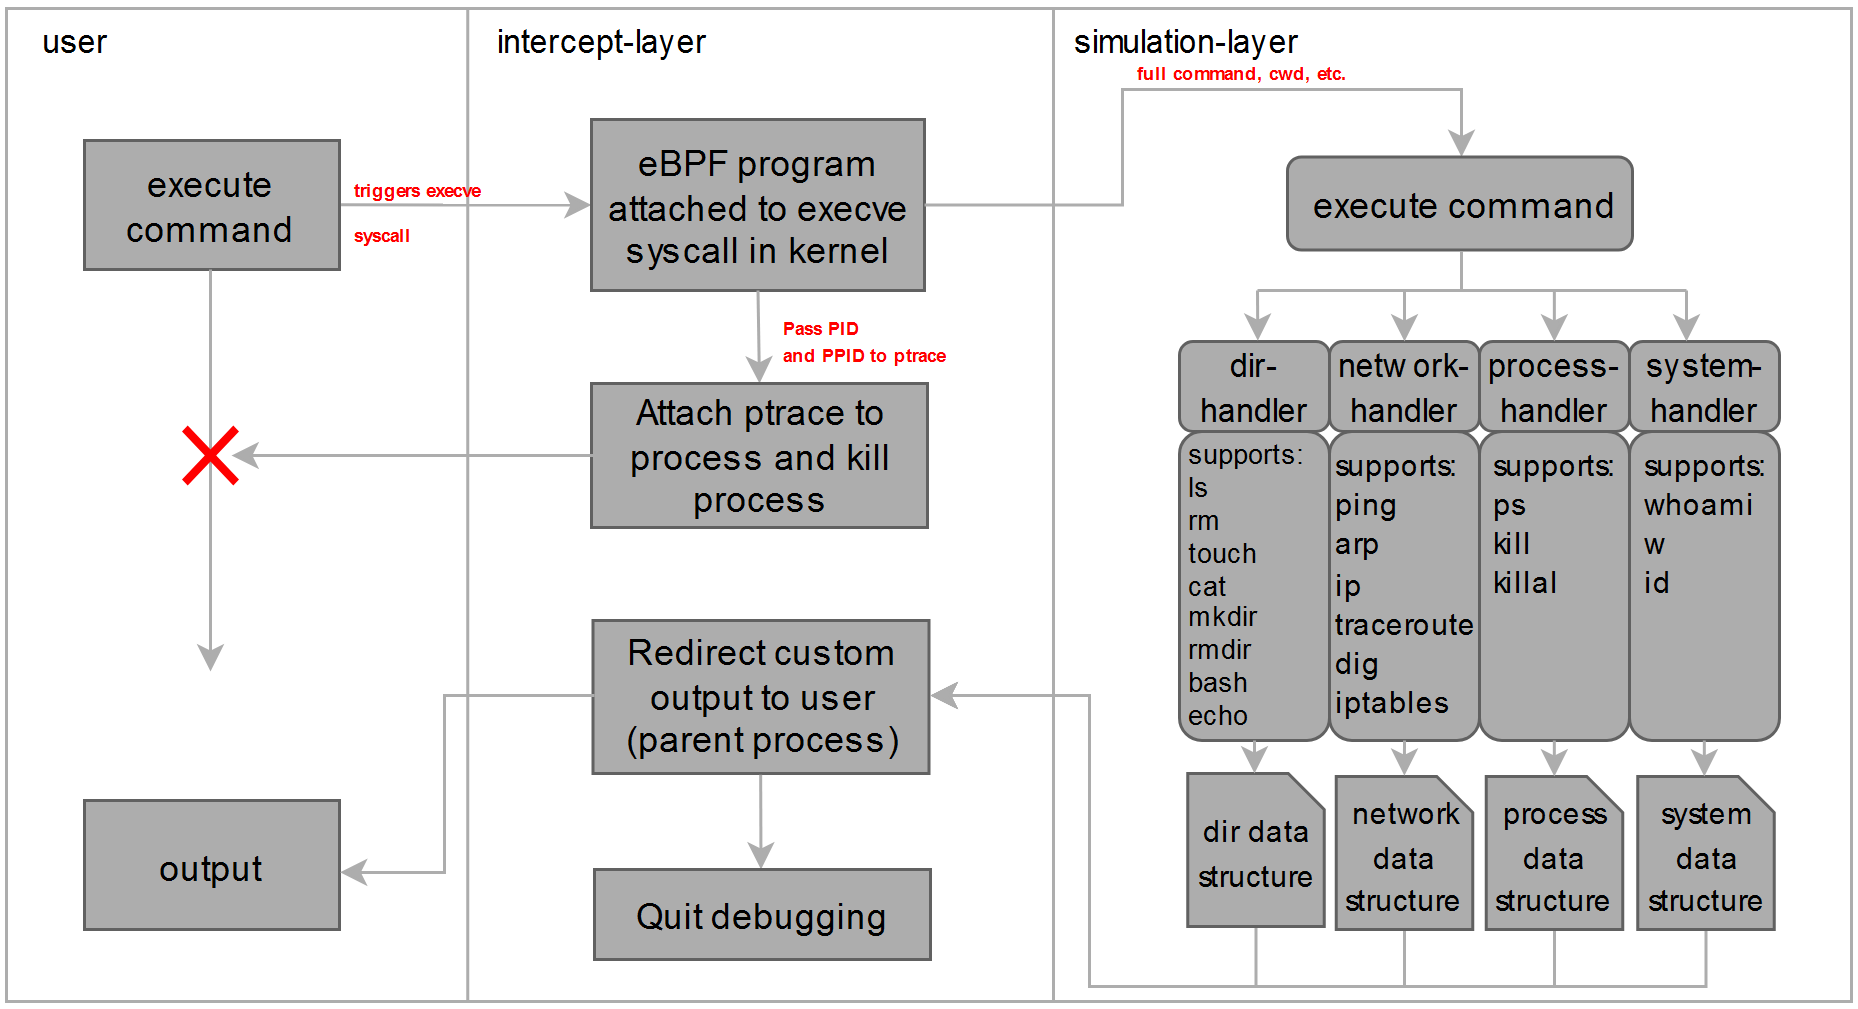
\includegraphics[width=1\linewidth]{bilder/pipeline.PNG}
    %\caption{Command pipeline}
    %\label{fig:enter-label}
%\end{figure}

\begin{figure}[H]
    \centering
    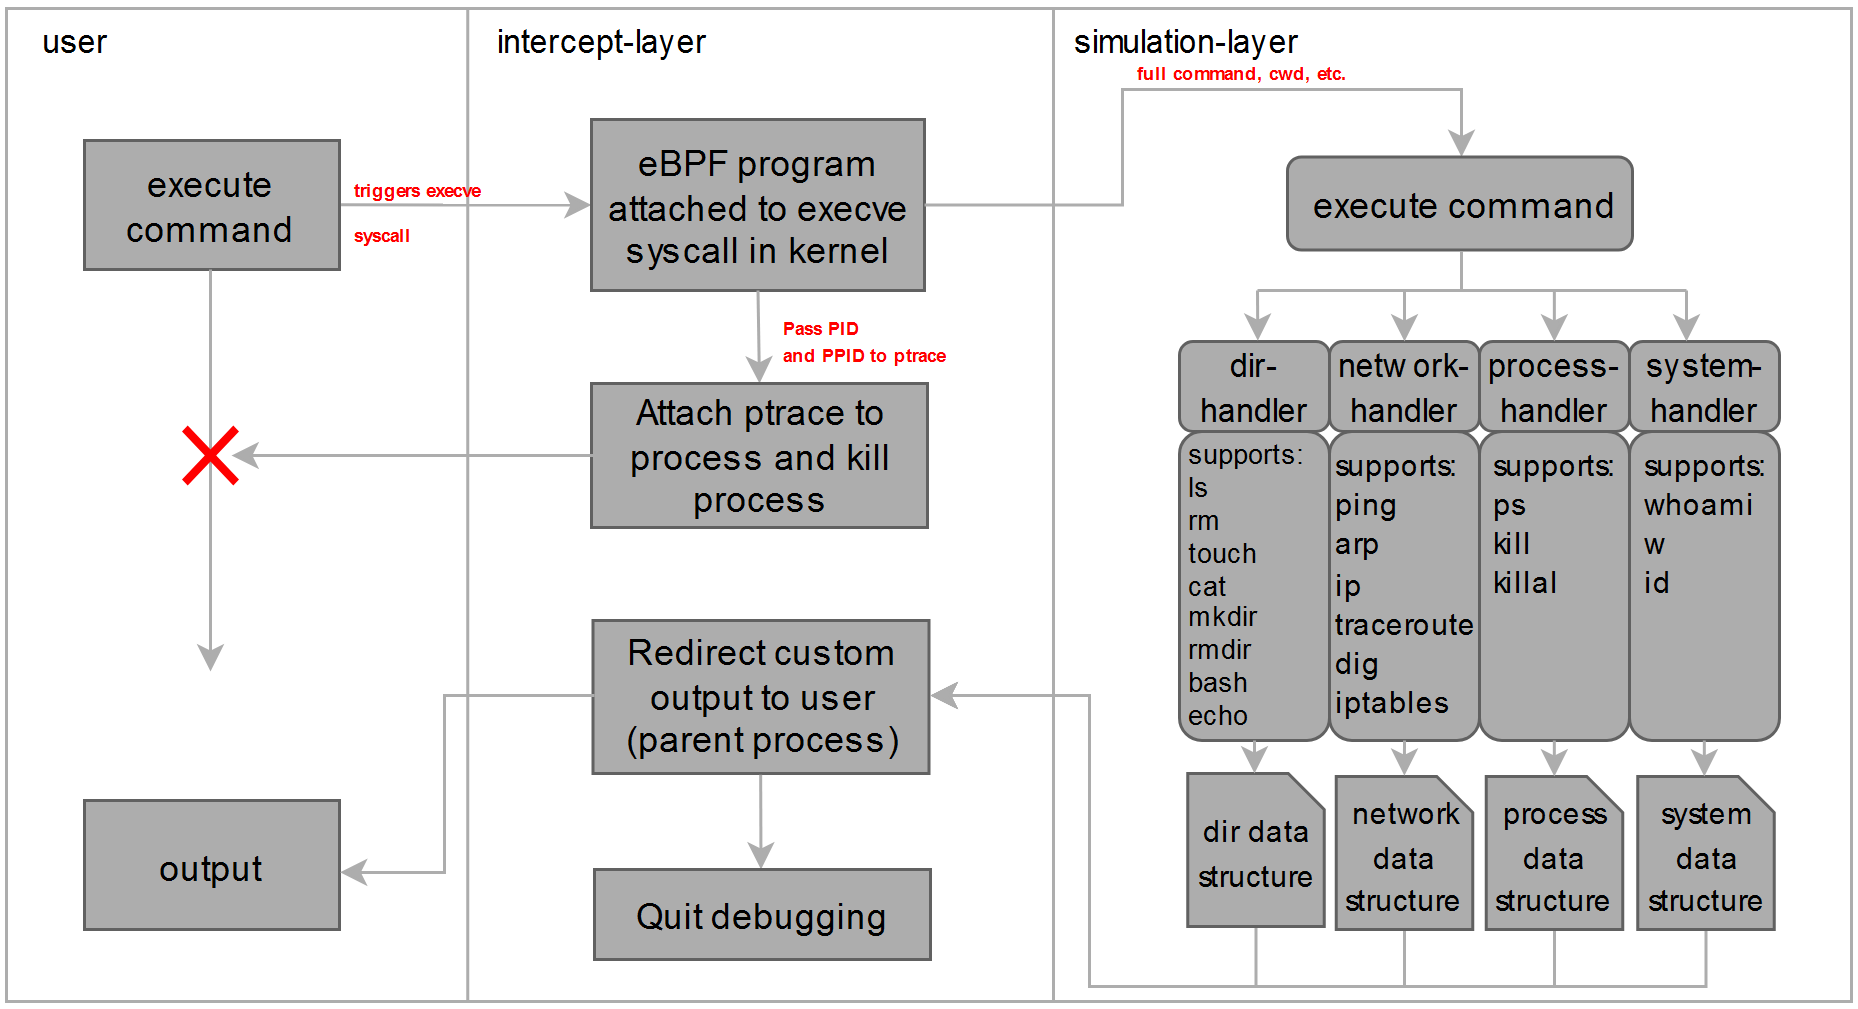
\includegraphics[width=1\linewidth]{bilder/pipeline.PNG}
    \caption{Command pipeline}
    \label{fig:enter-label}
\end{figure}


As shown in the graph, we use an intercept-layer to block the immediate execution of a command that is provided by a user. This layer is capable of calling APIs and deciding, which type of command it just intercepted. It can distinguish between directory-commands, network-commands, process-commands and system-commands. Examples for the different classes will be shown later.
After intercepting a command, it will call the corresponding API and deliver the command itself, all provided arguments and the current directory as a payload.

In the next step, the four handlers act as API endpoints and can react to a given input. For example a user might execute the ls-command. The "dir-handler" generates a simulated file system on program start using the data structure and can therefore apply a simulated ls-command on the virtual file system. The output is returned to the calling intercept-layer which will present it to the user. In theory the interception of commands and the simulated output can not be detected by the user.

\section{Command intercept}
As described in the previous section, the intercept-layer has two basic tasks. On the one hand, it has to trace and intercept all commands a user wants to execute. These commands have to be classified according to the four categories we defined (directory, network, process, system) and the corresponding API has to be called. On the other hand, the output of the called API has to be presented to the user in a way he can not distinguish it from a real output of the system.
\subsection{Tracing commands via eBPF}
\label{sub:ebpf}
To trace commands that are issued by the user we implemented and modified a eBPF program based on the exemplary "execsnoop.py" program that comes with the python bcc library \cite{execsnoop}. This program enables us to trace execution details of the "execve" system call that is triggered once the user commands are executed. Within the c-based eBPF program we use a structure to collect data such as the process ID, the parent process ID, the user id, the actual command as well as the arguments and other details like the return value. Furthermore, the user identifier 1000 of the user that is traced by the honeypot is hardcoded into the eBPF program. 
\begin{lstlisting}
# Define BPF program
bpf_text = """
#include <uapi/linux/ptrace.h>
#include <linux/sched.h>
#include <linux/fs.h>

#define ARGSIZE  128
#define UID_FILTER 1000

enum event_type {
    EVENT_ARG,
    EVENT_RET,
};

struct data_t {
    u32 pid;  
    u32 ppid; 
    u32 uid;
    char comm[TASK_COMM_LEN];
    enum event_type type;
    char argv[ARGSIZE];
    int retval;
};
\end{lstlisting}
To store events that can be read from userspace we make use of a BPF map.
\begin{lstlisting}
BPF_PERF_OUTPUT(events);    
\end{lstlisting}
Within the eBPF program we also utilize a function "syscall\_\_execvee" to trace the "execve" system call and capture the already mentioned parameters and store them in the BPF map. Helper functions such as "\_\_submit\_arg" and "submit\_arg" are responsible for reading and submitting arguments towards the map. Using the "BPF" class we then initialize the implemented eBPF program.
\begin{lstlisting}
b = BPF(text=bpf_text)
\end{lstlisting}
Afterwards, the function name of the "execve" system call needs to be resolved since these names can vary depending on the underlying kernel version. This ensures that we are tracing the correct system call.
\begin{lstlisting}
execve_fnname = b.get_syscall_fnname("execve")  
\end{lstlisting}
We then attach the eBPF program to the system call by utilizing bcc's "attach\_kprobe" which will execute the prior defined function "syscall\_\_execvee" once the "execve" system call is triggered.
\begin{lstlisting}
b.attach_kprobe(event=execve_fnname, fn_name="syscall__execve")
\end{lstlisting}
Lastly, we also attach a "kretprobe" which will capture returns of the system call and then execute the defined "do\_ret\_sys\_execve" eBPF function which simply captures the return value of the system call. 
\begin{lstlisting}
b.attach_kretprobe(event=execve_fnname, fn_name="do_ret_sys_execve")
\end{lstlisting}
All of the prior mentioned code samples are implemented within the main program "jamjar.py". Whenever the system call is triggered we execute the same routine which is implemented within the "proc\_event" function. This function processes the data that is returned by the eBPF program and therefore parses the process ID, which is required to intercept and kill the processes as well as the full commands which are needed for generating the fake output that is later returned to the user. Note that the "ptrace" debugger is attached to the target process as soon as the process ID has been parsed. Since the simulation layer also requires other data such as the current working directory for the command issued by the user, we derive such details from the file system entries for the traced processes within "/proc/<pid>/cwd". 

\newpage

\begin{lstlisting}
def proc_event():
    event = b["events"].event(data)

    if event.type == EventType.EVENT_ARG:
        argv[event.pid].append(event.argv)
    elif event.type == EventType.EVENT_RET:
        target_process = attach_ptrace(event.pid)
        argv_text = b' '.join(argv[event.pid]).replace(b'\n', b'\\n')
        cwd = os.readlink(f"/proc/{event.pid}/cwd")
        tty = os.readlink(f"/proc/{event.pid}/fd/0").replace("/dev/","")
        username = pwd.getpwuid(event.uid).pw_name
        # Getting cleaned command
        full_command,cmd_wo_args = cleaup_cmd(event.comm,argv_text)

        # Print event to console
        print_event(full_command,cwd,event.uid)
        # Handle commands
        event_handler(cmd_wo_args,event.pid,full_command,cwd,tty,event.ppid,username,target_process)
\end{lstlisting}
Once all the required details are parsed they are passed to a function "print\_event" which simply prints information regarding the traced command to the screen for logging purposes.
\bild{bilder/logoutput.png}{JamJar console output}{JamJar console output}
Furthermore, the parsed data is also passed to the function "event\_handler" which is responsible to call different subroutines which are implemented within "Subroutines.py" depending on the type of command that was issued by the user differentiating between directory, network and process commands.
\begin{lstlisting}
match comm:
    case ("ls"|"rm"|"touch"|"cat"|"echo"):
        PtraceSubroutines.dir_routine(pid,ppid,full_cmd,cwd,target_process)
        DEBUGGER.quit()
    case ("ping"|"arp"|"ip"|"traceroute"|"dig"|"iptables"):
        PtraceSubroutines.network_routine(pid,ppid,full_cmd,target_process)
        DEBUGGER.quit()
    case ("ps"|"kill"|"killall"):
        PtraceSubroutines.process_routine(pid,ppid,full_cmd,tty,username,target_process)
        DEBUGGER.quit()
    case ("whoami"|"w"|"id"):
        PtraceSubroutines.system_routine(pid, ppid, full_cmd, username, target_process)
        DEBUGGER.quit()
\end{lstlisting}
To constantly monitor for system call events we make use of a simple while-loop which then calls the "proc\_event" function once an event is triggered.
\begin{lstlisting}
b["events"].open_perf_buffer(proc_event)
    while True:
        try:
            b.perf_buffer_poll()
        except KeyboardInterrupt:
            exit()
\end{lstlisting}

\subsection{Intercepting and Killing Processes}
As mentioned in the previous section, as soon as the process id for the traced command is parsed we make use of the "ptrace" python library to attach to said process and put it in a halted state. This is required since processes for the traced commands exit rather quickly. Once "ptrace" is utilized to attach to the target process and all the required details are parsed within "jamjar.py" we move into the subroutines for the different commands within "PtraceSubroutines.py". This is where we kill the processes for the commands issued by the user and also pass the details to the simulation layer to generate the fake data and return it to the user. The different routines for the directory, network and process commands are very similar with the exception of commands such as "ping" or "traceroute" as they require time intervals for different sequences of output that is returned to the user. To establish a basic understanding of such routines we now detail the routine for network commands "network\_routine".
This function is called and passed with the parameters process id (pid), the parent process id (ppid), the full command (command) and the ptrace context (running\_process). 
\begin{lstlisting}
def network_routine(pid,ppid,command,running_process):
    ...
\end{lstlisting}
To first retrieve the fake output, we invoke a call to the simulation layer passing the full command.
\begin{lstlisting}
    cmd_output = CMD.invoke_network(command)
\end{lstlisting}
Now that the fake data has been generated we make sure to verify if the returned data is of type list, this would be the case if we need to delay the output for commands such as "ping" or "traceroute". If this is the case, we then call the helper function "write\_to\_proc" for each item in the list with a delay of one second. The helper function "write\_to\_proc" simply writes the fake output to the parent process of the issued user command which in this case is the tty of the user that issued the command.  
\begin{lstlisting}
    if type(cmd_output) == list:
            for n,item in enumerate(cmd_output):
                write_to_proc(item+"\n",str(ppid))
                if n < 5:
                    time.sleep(1)
        # Write modified output to target process
        else:
            write_to_proc(check_linebreak(cmd_output),str(pid))
        kill_and_quit(running_process,str(pid))
\end{lstlisting}
Once the fake output is returned to the user, we then call our second helper function\\ "kill\_and\_quit" which takes the "ptrace" context for the target process to then kill said process by sending a signal "SIGTERM". This then concludes the process of the intercept layer to trace and intercept user commands.

\newpage

\begin{lstlisting}
def kill_and_quit(process,pid):
    # Kill the process using SIGTERM
    process.kill(signal.SIGTERM)
    print(f"\t\\--> Attached to process [{pid}] and killed it!")    
\end{lstlisting}

\subsection{Challenges and Takeaways}
While implementing the intercept layer we came across multiple challenges. Originally we had in mind to perform this whole process by utilizing only eBPF programs. eBPF generally seems to be mainly used for its tracing capabilities and is therefore not meant to write within the kernel or modify system call return values and behavior to provide security within the kernel \cite{bcc}. Though it seems to be possible in certain edge cases it is not recommended as it would require changing certain kernel configurations which would put the availability of the operating system at risk.\\
While we opted to implement the actual interception and the termination of the processes via "ptrace" we originally attached to the command processes within "PtraceSubroutines.py" as it looked more reasonable at the time. This lead to the issue of race conditions as the processes for the user commands oftentimes already finished executing before we were able to attach to them. Therefore we decided to attach and halt the process as soon as we parsed the process ID via eBPF, this minimized the occurrence of race conditions significantly. Nevertheless, race conditions are still relevant as an attacker could simply use programs written in compiler languages such as C to outrun the execution flow of our python implemented honeypot.\\ Finally, we managed the termination of the user command processes by sending the "SIGTERM" signal. This would normally return signal messages such as "Terminated" to the user which would indicate that something went wrong while executing the command. To solve this we turned off the monitor mode for the target user by disabling it within the user's bash profile ".bashrc".
\begin{lstlisting}
export PROMPT_COMMAND='set +m'    
\end{lstlisting}


\newpage

\section{Command handler}
Next we have a look at the four command handlers.
As already mentioned in the theory-chapter, we can distinguish between four types of commands.
\textbf{Directory} related commands, \textbf{Network} related commands, \textbf{Process} related commands and \textbf{System} related commands.
Each command corresponds to a dedicated handler in the python code:
\begin{itemize}
    \item Directory-commands -> dir\_handler
    \item Network-commands -> network\_handler
    \item Process-commands -> process\_handler
    \item System-commands -> system\_handler
\end{itemize}

Each handler acts as an API-endpoint and needs some context to "execute" commands.
All four handlers define and build a simulated environment that can be used to execute the commands.
This environment is semi-persistent.
This means it is generated in a pre-defined state at program start and is completely discarded once the program stops.
So in case it is broken, all that has to be done is restart the program.
This could also be done periodically, for example every hour.

\subsection{Directory}
Simulating a directory is the most challenging part of the three handlers.
The most crucial aspect is designing a file system that on the one hand provides all the information that might be needed if a user executes a command (e.g \texttt{ls -a}).
On the other hand, commands like \texttt{rm} alter the file system, which needs to be taken into account and tracked. Further more, this simulated file system has to be efficient, as a delay of the output might be suspicious to an adversary.

To simulate the filesystem, we use Python objects.
Basis is the class \textbf{file}, which is used to represent a single "virtual" file.
Each file object has several attributes, such as permissions, owner and name.
One key aspect is the attribute "parent", which can be used to reference the parent object (a directory) of a file.
The init-method provides some default-values each time a new object of the class "File" is generated.

Directories can be seen as a special kind of files, because they share a lot of the same attributes.
Therefore we defined a new class "Dir" in "dir.py" which extends the class "File".
It also adds a new attribute to all objects of the class which is called "content".
This content-attribute holds a dictionary of all files and directories that are currently located in the directory.
In this case the key of the dictionary is the name of the object, the value is the object itself.
We used this approach to store the content rather than a simple list, because it allows for a quick and efficient navigation through the simulated fileystem. 

The last file that is needed before we focus on the directory-handler is called "helper.py".
This file contains helper-methods for all four handlers.
For example the method "create-fake-dir-data-helper" is used to create an initial fake directory structure with some data.
The dir-handler itself will call this function on initialization and set its root-point to the root of the generated fake file system.

Currently there are eight directory-commands with some common arguments supported.

\begin{table}[H]
    \centering
    \begin{tabular}{c|c|c}
        Command & Description & Supported Arguments\\
        \hline 
        ls & list directory contents & a / l / r\\
        rm & remove files or directory & r / f\\
        touch & create file or change file timestamp & -\\
        cat (see ch. \ref{sub:cat}) & list file content & -\\
        echo (see ch. \ref{sub:echo}) & displays text or command output & -\\
        mkdir & create directory & -\\
        rmdir & remove directory & -\\
        cd (see ch. \ref{sub:cd}) & change directory & -\\
    \end{tabular}
    \caption{Currently supported directory-commands}
    \label{tab:my_label}
\end{table}

Each command has a source-directory, where it is executed from (passed from the interception layer), and a target-directory (extracted from the command), where the command should be executed. Here are some examples:

\begin{table}[H]
    \centering
    \begin{tabular}{c|c|c}
        Command & Source directory & Target directory\\
        \hline
        user@comp:~\$ ls & /home/user & /home/user \\
        user@comp:~\$ ls /etc & /home/user & /etc \\
        user@comp:/home ls user & /home & /home/user \\
    \end{tabular}
    \caption{Possible context of the command "ls"}
    \label{tab:my_label}
\end{table}

Because of the many possible ways to execute a simple command such as \texttt{ls}, we have to think of a way to extract different sections of a command in a way that it is represented in a unified structure that can then be used to get the desired output.
The \texttt{ls} command for example can be split into four main points of interest:

\texttt{\color{blue}ls \color{red}-al \color{green}/home/user} executed in \texttt{\color{orange}/home}

\begin{enumerate}
    \item The command itself (\texttt{\color{blue}ls})
    \item Optional arguments (\texttt{\color{red}-al})
    \item Optional path. Can be an absolute or a relative path (\texttt{\color{green}/home/user})
    \item The directory the command was executed in (\texttt{\color{orange}/home})
\end{enumerate}

%%\todo[inline]{Zu viele Farben?}

Each of these sections, can hold a variety of different inputs, which change the output of the command.
Therefore, we need to look at each section and act accordingly.

To simplify this process, we first look at what variables are needed at the end to decide the output of the command.

For \texttt{ls} they are:

\begin{enumerate}
    \item The source directory
    \item The target directory
\end{enumerate}

With these two variables, we can always walk through the filesystem and find the directory the user wants to see.

By definition, every intercepted command is handed over with the source-directory as a parameter. Therefore this is fixed and can be used to find out the target-directory.
In the easiest case, the command does not contain a target-directory, meaning we can set the src-dir as the target-dir.
In case there is a parameter given as the target-directory, we are only interested in the object that represents the last folder in the given path.
For example, if the target-directory is given as \texttt{/a/b/c/d}, we only need the object of \texttt{d} to access its attributes like the "content", containing a dictionary of all files in that virtual folder.
To achieve this, the following small algorithm is used:

\begin{lstlisting}
for layer in src_dir_list:
    src_obj = src_obj.content[layer]
\end{lstlisting}

This algorithm on the virtual structure allows for an easy and efficient usage of the virtual file system.

If every aspect of the command has been taken into account, it is easy to determine the expected output.
For example if we know the source and target object of an ls command, we can find the corresponding object in our data-structure, which holds the desired data.
Finally the content of this object must be returned:

\begin{lstlisting}
for file in target_obj.content:
    output += file + " "
\end{lstlisting}

Additionally at this point further instructions and arguments that alter the display of the output would be taken into account.
This could for example be reversing the output string in case of the "-r" argument being present in the command.

Likewise when using the data-structure and helper functions to dissect a command, implementing further commands like \texttt{rm} and \texttt{touch} is very straight forward.

For example when using the data-structure and correct preprocessing of the command, a file can be deleted like the following.
This, of course, only represents the simplest case without any checks and arguments.

\begin{lstlisting}
src_obj.content.pop(target_file)
\end{lstlisting}

\begin{figure}[H]
    \centering
    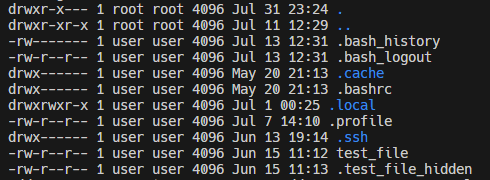
\includegraphics[width=1\linewidth]{bilder/ls.png}
    \caption{Simulated output of "ls -al /home/user"}
\end{figure}

\subsection{Network}
Currently there are six network-commands with some common arguments supported.

\begin{table}[H]
    \centering
    \begin{tabular}{c|c|c}
        Command & Description & Supported Arguments\\
        \hline 
        ip & interface related information & a / r / add / del\\
        ping & ping a host & c \\
        arp & view arp entries & d\\
        traceroute & see routers in the route to a host & - \\
        dig & retrieve DNS records for domains & x / v / A / AAAA\\
        iptables (see ch. \ref{sub:iptables}) & manage Linux network traffic rules & L / h / A / D / F\\
    \end{tabular}
    \caption{Currently supported network-commands}
    \label{tab:my_label}
\end{table}

On startup of the program we have to create a fake arp-table as well as a fake list of interfaces. This information is currently hard-coded but could be semi-randomized in the future. When the program is started, the methods "create-fake-arp-data-helper" and "create-fake-interface-data-helper" are execute which load the initial values for the arp-table and the list of interfaces from the file "interface.py" and "arp.py". After that, the environment is ready to handle network commands.

As already mentioned, we currently support the commands \texttt{ping}, \texttt{arp}, \texttt{ip}, \texttt{traceroute}, \texttt{dig} and \texttt{iptables} with some flags that are used often by a malicious actor.

On execution of the ping-command, our program will first check whether an ip-address is given as a parameter or a domain name. In the easiest case, an ip-address is given. The program will check, whether this ip-address is located in the same subnet as the the simulated interfaces using the python-library "ipcalc". If it is in the same subnet, the output of a normal ping-command will be handed back using a random value for the roundtriptime between 10 and 50 ms for each ping. By default, four pings are sent, but the user can adjust this number with the -c flag, specifying the desired number of pings.

\begin{figure}[H]
    \centering
    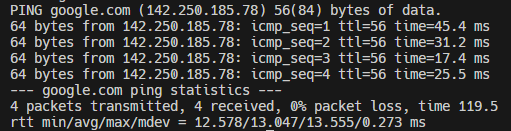
\includegraphics[width=1\linewidth]{bilder/ping.png}
    \caption{Simulated output of "ping google.com"}
\end{figure}

For each target that is pinged by the attacker, an entry in the arp-table should be established. Therefore we need to distinguish between local ip-adresses in the same subnet and addresses outside our subnet. If the ip-address is in the local subnet, an arp-entry for this ip-address is created. If the ip-address is outside the local network, an entry for the standard gateway is created.

The function also calculates realistic roundtrip time (RTT) statistics, including the minimum, average, maximum, and standard deviation of the RTT values. These computed statistics are displayed in the final output along with the RTT values for each individual ping.

Last but not least, if an attacker does not ping an ip-address but uses a domain name as a parameter, this address is translated into a real ip-address using the library "socket".

Similar to ping, traceroute shows information about the reachability of network devices, just with other faked data.

The arp-command can print the current arp-table or delete entries from this table. On startup, only the local address of the host is included in the arp-table. Whenever a user tries to ping a target as described in the previous section, this address is dynamically added to the arp-table. Of course these entries can also be deleted by the user.

The \textbf{ip} command is the most extensive command in the network handler.
It supports two \textbf{main arguments} which can be seen as two separate commands.

\begin{enumerate}
    \item \texttt{ip a}: Shows information about the network interface. 
    \item \texttt{ip r}: Shows information about set network routes.
\end{enumerate}

Both of these sub-commands support \texttt{add} and \texttt{del} as arguments.
Similar to the directory commands, a structure of objects is used in the back-end to store all necessary information about interfaces such as ip-address, gateway, hw-address, etc.

\begin{figure}[H]
    \centering
    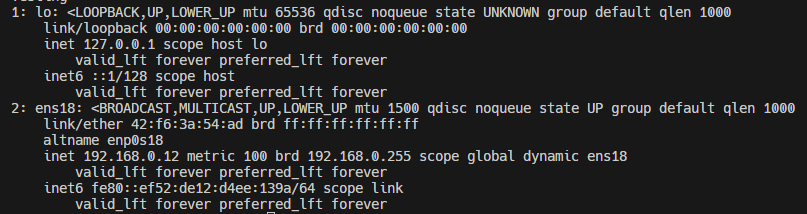
\includegraphics[width=1\linewidth]{bilder/ip.png}
    \caption{Simulated output of "ip a"}
\end{figure}

The \texttt{dig} command simulates the functionality of the widely used DNS querying tool, providing the ability to retrieve domain name system records and perform both forward and reverse lookups. The command accepts a domain name or IP address as input and processes it to generate a realistic DNS response. It supports a few flags to tailor the query, such as specifying whether to retrieve IPv4 (A) or IPv6 (AAAA) records or conducting reverse lookups for IP addresses.

When a domain name is queried, the program performs a forward lookup, resolving the name to its associated IP addresses. Depending on the flags used, the results include either IPv4 or IPv6 addresses, with simulated metadata such as TTL (Time To Live) and DNS query times. In cases where the domain cannot be resolved, the output indicates an appropriate error status, such as \textit{SERVFAIL}, replicating real-world DNS behavior. The generated response mirrors the typical output of the dig tool, including headers, sections for questions, answers, and additional information, along with metadata like the server address and the timestamp.

For reverse lookups, the command processes the provided IP address into the reverse DNS format (e.g., \textit{1.0.0.127.in-addr.arpa}) and attempts to resolve it back to a domain name. If the IP address can be resolved, the output includes a PTR record with the corresponding domain name. If the resolution fails, the result indicates a failure status, such as \textit{NXDOMAIN}, and includes relevant authority section data to simulate real-world behavior.

\begin{figure}[H]
    \centering
    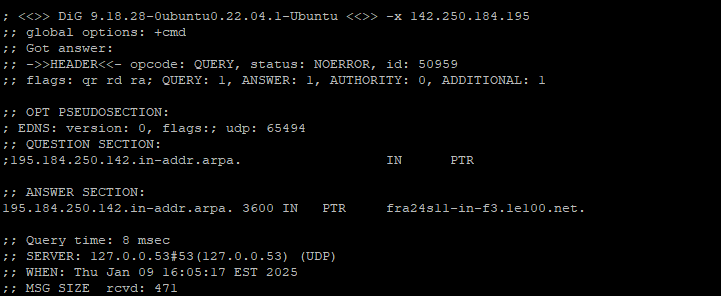
\includegraphics[width=1\linewidth]{bilder/rev-dns.png}
    \caption{Simulated output of "dig -x 142.250.184.195"}
\end{figure}


\subsection{Process}
Simulating process commands does also need a default list of simulated processes that run on the system. This initial list is copied from a running linux system in order to be as authentic as possible. Currently the process list with all its parameters is hard-coded but could be semi-randomized in the future. For example process-ids or cpu- and memory-usage could be given a random value on each program start. 

We identified the following commands to be important in an attack scenario: 

\begin{table}[H]
    \centering
    \begin{tabular}{c|c|c}
        Command & Description & Supported Arguments\\
        \hline 
        ps & Display processes & -a, -e, -A, -f, -C, -u, a, u, x \\
        kill, killall  & Terminate process & - \\
    \end{tabular}
    \caption{Currently supported process-commands}
    \label{tab:my_label}
\end{table}


%https://man7.org/linux/man-pages/man1/ps.1.html
The most difficult one to implement is \texttt{ps}. It reports a snapshot of the current processes.
The version of \texttt{ps} that is mimicked has three different syntax options: UNIX-options that can be grouped and use a dash in front of the letter; BSD options which also can be grouped but do not use a dash and GNU options that use two dashes\cite{noauthor_ps1_2024}.
Our implementation includes some Unix options and some BSD options. 

Every \texttt{ps} call from the intercept layer includes the current terminal and the current user ID. With this information an accurate representation of the processes can be generated and returned. Without a given parameter, \texttt{ps} hands back a list of all processes currently running by the user who executes the command and the current terminal the command is executed in\cite{noauthor_ps1_2024}. In our implementation all process objects are filtered by the user id (UID) and the terminal (TTY) that is send by the intercept layer:

\begin{lstlisting}
    if not args_str:
        for process in self.output: # none
            if (process.tty == tty or process.tty == "pts/0") 
            and process.uid == uid:
                processes.append(process)
\end{lstlisting}


The process objects that fit that criteria are selected and their information is turned into an output that looks similar to the original output using .format():

\begin{lstlisting}
    for process in processes:
        process_list.append([process.pid, process.tty, process.stat, 
        process.time[-4:], process.ucmd])

        process_list = [["PID", "TTY", "STAT", "TIME", "COMMAND"]] + 
        sorted(process_list, key=lambda x: x[0])

        for row in process_list:
             output+= "{:>6} {:<8} {:<4} {:<4} {:<4}\n".format(*row)
\end{lstlisting}

The process information that is presented by \texttt{ps} without a parameter includes the process ID (PID), the terminal associated with the process (TTY), the accumulated CPU time in [DD-]hh:mm:ss format (TIME) and the executable name (CMD)\cite{noauthor_ps1_2024}. As seen in Figure \ref{fig:outputps} the layout of the simulated output resembles the real output, but it is possible to manipulate the processes that are shown. The following options follow a similar algorithm simply changing the filtered attributes and the format of the output for each parameter. 

\begin{figure}[H]
    \centering
    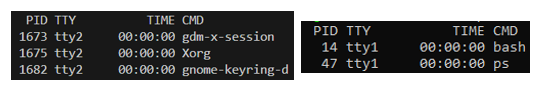
\includegraphics[width=1\linewidth]{bilder/real_and_fake_ps.png}
    \caption{Simulated output of "ps" (left) and real output (right)}
    \label{fig:outputps}
\end{figure}

The Unix options that are included in our implementation are "-a", "-e/-A", "-f", "-C" and "-u" and most combinations of multiple parameters. \texttt{ps -a} displays all processes but excludes all session leaders. Session leaders have the same process Id and Session ID. \texttt{ps -e}  or \texttt{ps -A} display all processes of the system without any filters. \texttt{ps -C} is able to filter all processes by the process name\cite{noauthor_ps1_2024}.

\begin{figure}[H]
    \centering
    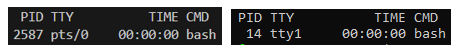
\includegraphics[width=1\linewidth]{bilder/real_and_fake_psC.png}
    \caption{Simulated output of "ps -C bash" (left) and real output (right)}
    \label{fig:enter-label}
\end{figure}

Another filter option is \texttt{ps -u}. This parameter filters all processes by a user Id and only displays processes belonging to that user\cite{noauthor_ps1_2024}.

The last Unix parameter that is implemented is "f". It is able to display additional information about the processes by adding additional columns. The information includes the user ID, process ID, parent process ID, CPU utilization in percent, terminal associated with the process, elapsed CPU utilization time for the process and the name of executable command\cite{noauthor_ps1_2024}.

\begin{figure}[H]
    \centering
    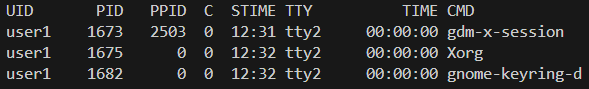
\includegraphics[width=1\linewidth]{bilder/fake_psf.png}
    \caption{Simulated output of "ps -f"}
    \label{fig:enter-label}
\end{figure}

This option only changes the format of the output and not the displayed selection of processes. It can also be combined with other parameters. For example it is possible combine "-f" and "-u" to search for a specific user ID and display the selected with more information as seen in Figure \ref{fig:outputpsuser}. 

\begin{figure}[H]
    \centering
    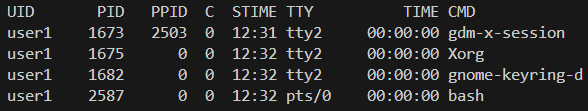
\includegraphics[width=1\linewidth]{bilder/fake_psfu.png}
    \caption{Simulated output of "ps -fu user1"}
    \label{fig:outputpsuserl}
\end{figure}

The BSD-options that are implemented include "a","x", "u". \texttt{ps a} displays all processes in the current terminal but has a different layout additionally displaying the process state codes (STAT) and the long name of the executable command \cite{noauthor_ps1_2024} as seen in Figure \ref{fig:outputpsa}. 

\begin{figure}[H]
    \centering
    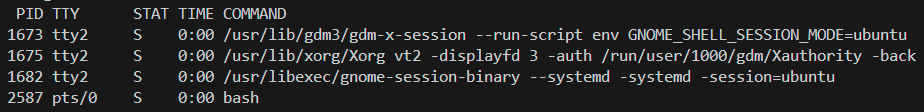
\includegraphics[width=1\linewidth]{bilder/fake_psa.png}
    \caption{Simulated output of "ps a"}
    \label{fig:outputpsa}
\end{figure}

The option \texttt{ps x} shows all processes of the current user, but combined with "a" it displays all processes in the system. The option "u" displays a user-oriented format with additional information like the used ID, cpu utilization of the process in "\#\#.\#" format, ratio of the process's resident set size to the physical memory on the machine, virtual memory size of the process in KiB, resident set size and the start time of the process. The popular combination of all three \texttt{ps aux} shows all processes with additional information \cite{noauthor_ps1_2024} as seen in Figure \ref{fig:fakepsaux}.

\begin{figure}[H]
    \centering
    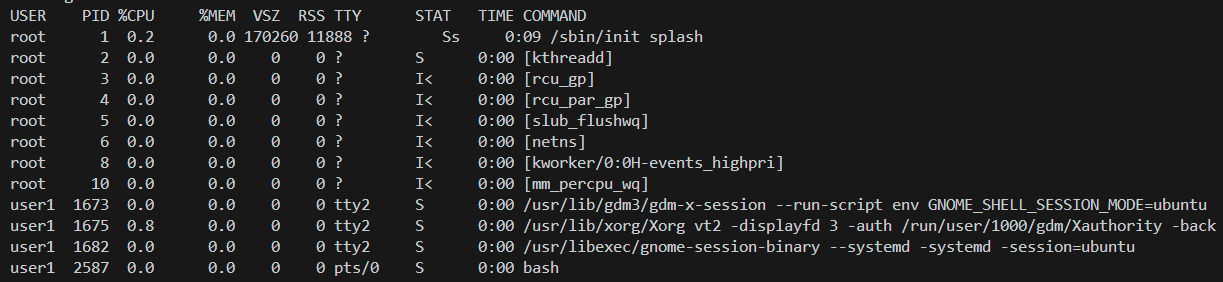
\includegraphics[width=1\linewidth]{bilder/fake_psaux.png}
    \caption{Simulated output of "ps aux"}
    \label{fig:fakepsaux}
\end{figure}

The commands \texttt{kill} and \texttt{killall} can used to terminate processes\cite{kill}\cite{noauthor_killall1_2023}. This is done by simply removing entries from the list of simulated processes. \texttt{kill} is used with a process ID to remove the process with this ID\cite{kill}.\texttt{killall} uses the executable command to terminate a process\cite{noauthor_killall1_2023}.

\begin{lstlisting}
for process in self.output:
            if process.pid == target_process:
                self.output.remove(process)
                valid_arg = True
\end{lstlisting}

To check weather the process was removed a \texttt{ps} command can be submitted before and after submitting \texttt{kill} or \texttt{killall}. If the argument is not valid an error message is displayed that resembles a real error message.

\subsection{System}
The system command handler is responsible for simulating common system-related commands such as \texttt{whoami}, \texttt{id}, and \texttt{w}. These commands are used to retrieve information about the current user and system status, often employed in reconnaissance or debugging scenarios. While their current implementation is hardcoded to provide consistent and predictable outputs, they could be extended in the future to include semi-randomized elements for greater realism.

Currently there are only three basic system-commands supported.

\begin{table}[H]
    \centering
    \begin{tabular}{c|c|c}
        Command & Description & Supported Arguments\\
        \hline 
        whoami & displays the current username & -\\
        id & shows user and group IDs & - \\
        w & lists active user session details & -\\
    \end{tabular}
    \caption{Currently supported system-commands}
    \label{tab:my_label}
\end{table}

The \texttt{whoami} command simply returns the current username, which is passed to the event handler upon initialization. The \texttt{id} command provides details about the user’s ID, group ID, and associated groups, with static values reflecting a typical Linux environment. The \texttt{w} command simulates an active session, displaying system uptime, load averages, and user activity, including login times, idle durations, and the currently executed command. Although the \texttt{w} command currently uses fixed data, attributes such as system uptime, load averages, or idle times could be randomized in the future to enhance authenticity.

\begin{figure}[H]
    \centering
    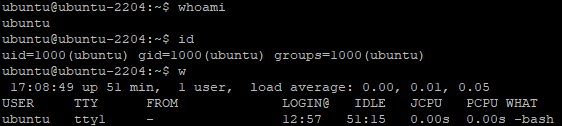
\includegraphics[width=1\linewidth]{bilder/system.png}
    \caption{Simulated output of system commands}
    \label{fig:enter-label}
\end{figure}

The underlying implementation relies on a unified interface for command execution. When a command is issued, the handler identifies the requested command, extracts the relevant parameters, and invokes the corresponding helper function to produce the simulated output. This modular approach allows for flexibility and extensibility, making it easy to add additional system commands in the future.

\section{Logging}
Every command intercepted and processed by the handlers is logged in a central log-file. This is done using the python-library "logging". The basic configuration of the logging is executed once on program startup. It is persistent, so even if the program ends and is run again, the new log entries will be appended to the existing file. It needs the following configuration parameters: \newline

\begin{itemize}
    \item level: Sets the threshold for this logger. Messages which are less severe than the given level, in this case "INFO", will be ignored. Using this level-model given by the library means we can mark some dangerous commands in the log-file.
    \item format: The format is set as "Year-Month-Day Hours:Minutes:Seconds Log-Level Message", where the message-parameter contains the whole intercepted command including all parameters.
    \item datefmt: The date format described in the format-section.
    \item filename: As this project is about a honeypot-system, the log-file got the related name "jamjar".
\end{itemize}

\begin{lstlisting}
    logging.basicConfig(
        level=logging.INFO,
        format="%(asctime)s %(levelname)s %(message)s",
        datefmt ="%Y-%m-%d %H:%M:%S",
        filename="jamjar.log"
    )
\end{lstlisting}

\section{Additional Commands}

\subsection{cd}
\label{sub:cd}

Like described in section \ref{sub:ebpf}, the interception of commands is currently achieved primarily by monitoring \texttt{execve} system calls using eBPF code. While this approach works well for commands that spawn new processes, it does not cover built-in commands like \texttt{cd}, which do not trigger an \texttt{execve} call. This limitation causes, among other things, issues when navigating directories within the honeypot. For example, if a user creates a fake directory using \texttt{mkdir} and subsequently attempts to navigate into it using \texttt{cd}, the command is executed on the host system rather than being properly handled within the honeypot environment. This results in errors, as the directory only exists in the honeypot's simulated file system.

To address this, the first step was analyzing the behavior of the \texttt{cd} command to understand which system calls it invokes. This was done using tools like \texttt{strace}, which traces the system calls made by a bash process executing for example the \texttt{cd} command. The output revealed that \texttt{cd} does not call \texttt{execve}, but instead relies on the \texttt{chdir()} system call to change the current working directory.

\begin{lstlisting}
$ strace -f bash -c "cd /home" 
... 
chdir("/home")                   = 0
... 
\end{lstlisting}

The above output, captured with \texttt{strace}, demonstrates that \texttt{chdir()} is the key system call responsible for directory changes. To enhance the honeypot's capabilities, we extended our eBPF code to intercept \texttt{chdir()} calls. Below is the code snippet used for this purpose:

\begin{lstlisting}
int syscall__chdir(struct pt_regs *ctx, const char __user *argv) {
    struct data_t data = {};
    struct task_struct *task;

    u32 uid = bpf_get_current_uid_gid() & 0xffffffff;
    if (uid != UID_FILTER) {
        return 0;
    }

    data.pid = bpf_get_current_pid_tgid() >> 32;
    data.uid = uid;

    task = (struct task_struct *)bpf_get_current_task();
    data.ppid = task->real_parent->tgid;
    bpf_get_current_comm(&data.comm, sizeof(data.comm));
    data.timestamp = bpf_ktime_get_ns();
    data.type = EVENT_CD;
    bpf_probe_read_user(&data.argv, sizeof(data.argv), argv);
    events.perf_submit(ctx, &data, sizeof(data));
    return 0;
}
\end{lstlisting}

This probe allows the honeypot to detect when a directory change is attempted, capturing both the target directory and other relevant data for logging or simulation purposes.

To simulate the behavior of the \texttt{cd} command, we also needed to determine the current working directory of the process executing the command. This is crucial to validate whether the target directory is reachable from the current directory within the honeypot's virtual file system. Although this functionality is not yet fully implemented, the foundation is in place to enable future enhancements. Logs already provide feedback on whether a directory change would be successful in the simulated environment.

Another consideration is the terminal prompt itself. In a real Linux environment, the prompt reflects the current working directory, such as:

\texttt{ubuntu@ubuntu-2204:/home\$}

One possible approach to addressing this issue could be to fake the prompt within the honeypot to align with the simulated environment. This could be achieved by modifying the \texttt{PS1} variable in the \texttt{.bashrc} file. However, such changes should be applied dynamically to ensure they only affect sessions running within the honeypot.

While the current implementation serves as a foundational layer, it highlights several areas for future work, including:

\begin{itemize}
    \item Fully integrating the \texttt{cd} command into the honeypot’s virtual file system.
    \item Simulating or manipulating the terminal prompt to reflect the honeypot’s state dynamically.
    \item Handling edge cases, for example symlinks, to improve authenticity.
\end{itemize}

To illustrate the issue with the \texttt{cd} command, we created a directory within the honeypot's simulated file system. From the attacker's perspective, the directory creation appears successful, but attempting to change into the newly created directory fails. This happens because the \texttt{cd} command is still executed on the host system, where the directory does not exist. Below is a screenshot showing the attacker's terminal output during this process:

\begin{figure}[H]
    \centering
    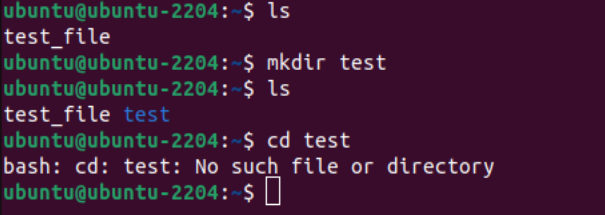
\includegraphics[width=1\linewidth]{bilder/attacker.png}
    \caption{Attacker's perspective: Attempt to change into a fake directory fails.}
\end{figure}

In contrast, the honeypot's logs accurately reflect the expected behavior within the simulated environment. These logs confirm that the directory change would have been successful if it had been handled entirely within the honeypot. The logs include details about the intercepted \texttt{chdir()} system call, the target directory, and whether the operation was valid. The screenshot below shows the corresponding log entry:

\begin{figure}[H]
    \centering
    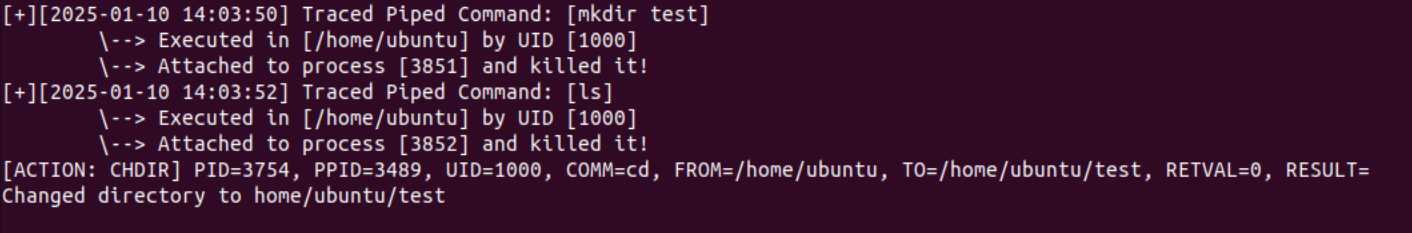
\includegraphics[width=1\linewidth]{bilder/logs.png}
    \caption{Honeypot logs: Successful directory change simulation.}
\end{figure}

This example highlights the current limitation of executing \texttt{cd} on the host system rather than fully within the honeypot and demonstrates how the extended eBPF code and logging provide accurate simulation data for future enhancements.

\subsection{Piped Commands}
\label{sub:pipes}

The goal of implementing piped commands in the honeypot was to simulate Linux-like behavior when executing multiple commands chained together using the pipe symbol (\texttt{|}). However, due to the nature of how piped commands operate and the honeypot's current architecture, several challenges arose, requiring additional analysis and foundational improvements for future enhancements.

Piped commands execute each command in the chain as a separate process, with the output of one command serving as the input to the next. For example, a command like \textbf{\texttt{touch test | ls}} spawns two distinct processes:

\begin{enumerate}
    \item \texttt{touch test}, which creates a file named \texttt{test}.
    \item \texttt{ls}, which lists the contents of the directory, including the newly created \texttt{test} file.
\end{enumerate}

The pipe ensures that the output of the first process (\texttt{touch test}) is directly connected to the input of the second process (\texttt{ls}). This sequential data flow makes it difficult to handle piped commands in the honeypot, as the current implementation processes one command at a time without considering the interdependence of outputs and inputs in a pipeline.

Using \texttt{strace}, the behavior of piped commands was analyzed. The command produced output revealing a \texttt{pipe2} system call, which is used to establish the communication channel between commands in the pipeline:

\begin{lstlisting}
$ strace -f bash -c "touch test | ls"
... 
pipe2([3, 4], 0)                   = 0
... 
\end{lstlisting}

This discovery highlighted that the honeypot needed to intercept \texttt{pipe2} system calls in addition to the existing \texttt{execve} monitoring. To address this, the eBPF code was extended as follows:

\begin{lstlisting}
int syscall__pipe2(struct pt_regs *ctx, int __user *pipefd)
{
    struct data_t data = {};
    u32 uid = bpf_get_current_uid_gid() & 0xffffffff;
    if (uid != UID_FILTER) {
        return 0;
    }

    data.pid = bpf_get_current_pid_tgid() >> 32;
    data.uid = uid;
    data.timestamp = bpf_ktime_get_ns();
    bpf_get_current_comm(&data.comm, sizeof(data.comm));
    data.type = EVENT_PIPE;
    events.perf_submit(ctx, &data, sizeof(data));
    return 0;
}
\end{lstlisting}

This enhancement enabled the honeypot to detect when a pipeline was initiated, allowing further logic to handle piped commands.

Despite detecting the \texttt{pipe2} system call, several challenges remained:

\begin{enumerate}
    \item Command Sequencing: Since each command in the pipeline spawns a separate process, there is no straightforward way to determine the total number of commands in the pipeline or their exact order. The \texttt{execve} calls are processed one by one, meaning the honeypot would process and output each command individually, breaking the sequential flow required for a proper pipeline simulation.

    \item Simulating Outputs and Inputs: The honeypot needs to store the output of each command in the pipeline and pass it as input to the next. Initially, a \texttt{piped} flag was introduced, which, when set to \texttt{True}, prevented the immediate output generation. Instead, command outputs were temporarily stored in a buffer. The idea was to wait until the final command in the pipeline was reached before processing the output.

    \item Identifying the Final Command: A significant challenge was determining when the last command in the pipeline had been reached. Since the honeypot processes each \texttt{execve} call independently, there was no clear indicator marking the end of the pipeline. The \texttt{pipe2} system call does not provide information about how many commands are connected via pipes. To address this, a counter was implemented to track the number of commands. For simplicity, an initial predefined maximum of two commands was set, and once this limit was reached, the pipeline processing logic was triggered.

    \item Re-execution and Ordering: Another approach involved collecting all processes in the pipeline, sorting them for example by process ID (PID) to ensure the correct order, and then re-executing the commands in sequence. This method faced issues as many processes had already terminated by the time the re-execution logic was applied, making it impossible to write outputs back to their respective \texttt{/proc/<pid>/fd/1} files.
\end{enumerate}

The current implementation focuses on handling up to two commands in a pipeline. Outputs are buffered, and the pipeline's results are written to the final process in the chain. However, due to the nature of piped commands and the limitations of the current architecture, several issues persist:

\begin{itemize}
    \item Processes often terminate too quickly, making it almost impossible to reliably attach to them using \texttt{attach\_trace}. As a result, capturing their outputs or integrating them into the pipeline simulation frequently fails.
    \item The reordering of processes is error-prone and does not always align with real-world behavior.
    \item Simulating complex pipelines with more than two commands remains infeasible due to these challenges, as the current implementation struggles to handle interdependent processes in a coordinated manner.
\end{itemize}

The earlier approach of re-executing all processes in the correct order would theoretically allow the honeypot to handle pipelines with an arbitrary number of commands. However, due to the issues with terminated processes and inaccessible file descriptors, this method was ultimately abandoned in favor of the simpler two-command limit.

Due to these challenges, parts of the code have been commented out and are currently non-functional. These sections, however, serve as a foundation for future improvements. They highlight key areas where the logic could be refined to achieve a more reliable and accurate simulation of piped commands. While the current logic is not yet robust enough for consistent and trustworthy results, it provides valuable insights and a framework for developing a fully functional implementation.

\subsection{iptables}
\label{sub:iptables}

The \texttt{iptables} command simulates the basic functions of the Linux command \texttt{iptables}, which makes it possible to use network filters. Therefore, a central class, Iptables, is used to manage and store the groups (chains) and the related rules. The predefined chains in this implementation are INPUT, FORWARD, and OUTPUT. These chains are managed by a class located in the helper folder, specifically in the \texttt{iptable.py} file. This class is designed to efficiently handle the storage, retrieval, and management of rules.

The class contains the following functions:

\begin{itemize}
    \item add\_rule(self, chain, source, destination, protocol, source\_port, destination\_port, action): This function makes it possible to create new rules for the various chains.
    \item remove\_rule(self, chain, source, destination, protocol, source\_port, destination\_port, action): This function allows you to delete certain rules.
    \item list\_rules(self): This function lists all existing rules together with their chains.
    \item clear\_chain(self, chain): This function can be used to empty a chain.
    \item clear\_all(self): This function can be used to remove all existing rules.
    \item rule\_exists(self, chain, source, destination, protocol, source\_port, destination\_port, action): This function can be used to check whether a specific rule exists or not.
\end{itemize}

It supports various arguments like -L, -h, -help, -A, -D and -F. The functions of these arguments are explained below:

\begin{itemize}
    \item -L: This argument allows you to output the current rules and chains.
    \item -h \& –help: This argument can be used to output the help overview.
    \item -A: This argument can be used to create a new rule.
    \item -D: This argument allows you to delete a rule. It checks whether the rule to be deleted does exists.
    \item -F: With this argument, either all chains or only a specific chain can be emptied by passing a chain name.
\end{itemize}

For example you can display all chains and rules with the command \textbf{\texttt{iptables -L}}:

\begin{figure}[H]
    \centering
    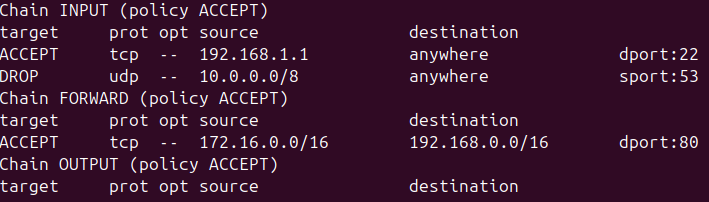
\includegraphics[width=1\linewidth]{bilder/output-iptables.PNG}
    \caption{iptables output}
\end{figure}

To block outgoing ICMP traffic and prevent pings, you can use the following approach:

For example, executing the command \textbf{\texttt{iptables -A OUTPUT -p icmp -j DROP}} will add a rule to the OUTPUT chain that blocks all outgoing ICMP packets. As a result, if you try to ping a domain, like ping google.com, the request will fail because the ICMP packets are dropped.

\begin{figure}[H]
    \centering
    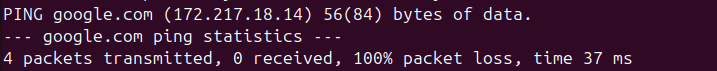
\includegraphics[width=1\linewidth]{bilder/ping_fail.PNG}
    \caption{ping fail}
\end{figure}

\subsection{cat}
\label{sub:cat}
The \texttt{cat} command replicates the core functionality of the Linux \texttt{cat} command, enabling the content of a file to be displayed directly in the terminal. In this implementation, simulated files and their contents are represented as file objects created using the touch command. The contents of each file are stored in the file\_content variable within the corresponding class, ensuring efficient access and management of file data.

When executing the \texttt{cat} command, the process begins by checking whether a file name has been provided as an argument. If an argument is supplied, the command then verifies whether the specified file exists. Once confirmed, it determines if the argument refers to a file or a folder. If the argument equals a folder, an error message is displayed, indicating that directories cannot be processed. However, if the argument corresponds to a valid file, the command reads and displays its content directly in the terminal.

For instance, if you use the \texttt{cat} command to display the contents of a script, the output will show the file's text as follows:

\begin{figure}[H]
    \centering
    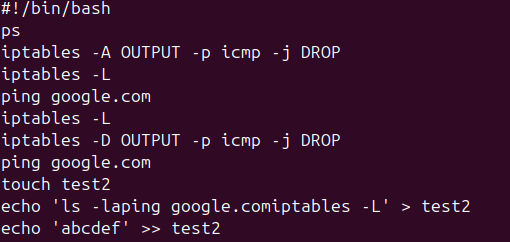
\includegraphics[width=1\linewidth]{bilder/cat.PNG}
    \caption{Simulated output of cat command}
\end{figure}

\subsection{bash}

The bash(self, args, scr\_dir) function provides the capability to execute scripts with various contents in a secure and controlled environment. To run a script, the command \textbf{\texttt{./{filename}}} is used. When executed, the function first checks whether the specified file exists. If the file is not found, an appropriate error message is displayed. However, if the file exists, the function verifies whether it is an executable file and whether the required permissions are in place for execution.

If the necessary permissions are granted, the script's execution begins. The script's content is processed line by line, with each line sent for execution individually. If the first line of the script contains a shebang (e.g., \#!/bin/bash), it is recognized and skipped to prevent errors during execution. Once the shebang is processed, each command in the script is passed sequentially to the execute\_command(self, command, src\_dir) function, which is placed in the \texttt{scripts.py} file within the helper folder. This modular approach ensures a robust and error-free execution of scripts.

Additionally, commands like \texttt{echo} can include text inside quotation marks (' or "), which might contain line breaks. These line breaks are treated as part of the text, and everything inside the quotation marks is processed as a single unit to avoid errors.

\begin{figure}[H]
    \centering
    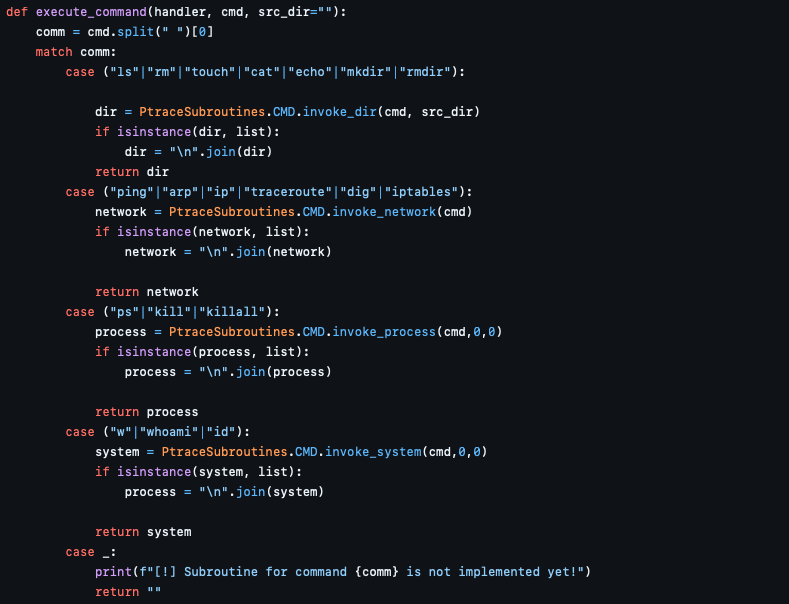
\includegraphics[width=1\linewidth]{bilder/execute_command.PNG}
    \caption{Execute Command function}
\end{figure}

The execute\_command function is designed to process individual commands without creating a separate process, returning the result of each command as a string. These output strings are collected by the bash function, merged into a single output, and then displayed in the terminal.

The execute\_command function takes two arguments: cmd (the command to execute) and an optional src\_dir (the source directory, if required). The function operates by analyzing the main command (the first part of cmd), identified by splitting the string at the first space. Based on this, the command is routed to the right subroutine corresponding to its type. This makes sure that each command is handled properly and efficiently, and its output is combined smoothly into the final result provided by the bash function.

For example, if you execute a script that has the following content:

\begin{lstlisting}
#!/bin/bash
iptables -A OUTPUT -p icmp -j DROP
iptables -L
ping google.com
iptables -D OUTPUT -p icmp -j DROP
iptables -L
ping google.com
\end{lstlisting}

The individual commands are executed sequentially. First, a new iptables rule is added to block all ICMP packets. Afterward, the current iptables rules are listed to confirm that the new rule has been successfully created. Next, a ping to google.com is attempted, demonstrating that the rule is functioning correctly by dropping the ping request. Finally, the rule is removed, the updated rules are displayed, and a subsequent ping is performed to verify that ICMP traffic is working again.

The output appears as follows:

\begin{figure}[H]
    \centering
    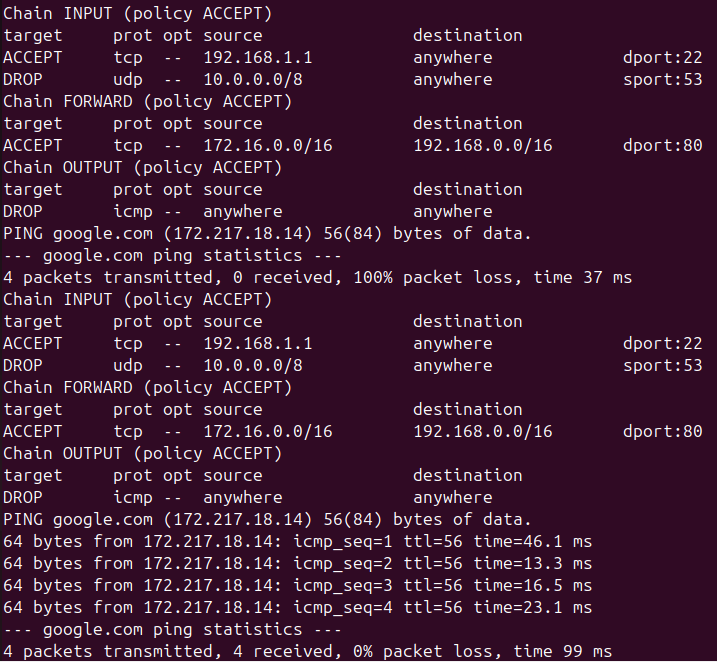
\includegraphics[width=1\linewidth]{bilder/script.PNG}
    \caption{Simulated output of "script"}
\end{figure}

\subsection{echo}
\label{sub:echo}
The \texttt{echo} command is not fully implemented as it is a shell build-in command by default. Built-ins are processed directly by the shell itself and are not executed as independent executable files in the file system. That's why the \texttt{echo} command does not work completely. 
In contrast, /bin/echo works because it is an independent executable file that is located directly in the file system. When using /bin/echo, a new process is started that executes system calls such as execve, allowing the command to be monitored and traced. However, using only \texttt{echo} results in the shell's built-in being executed, which is processed internally and does not generate comparable system calls.

If the \texttt{echo} command is implemented in a script, the built-in echo also works reliably. This is because executing the bash function simulates the individual commands within the script without creating a process.

The echo function starts with a check of the arguments (args). If no arguments are specified, a line break (\textbackslash n) is simply returned, as is the case with the original \texttt{echo} command.

It is then checked whether redirection characters such as \texttt{>} or \texttt{>>}  are contained in the arguments. If no redirection is specified, the function simply returns the arguments as a linked string. If redirection characters are found, the function attempts to write the text to the specified file. If one of these arguments is found, the function checks if the target file exists. If the file exists, the new text is written to the contents of the file. If the file does not exist, the function returns an error message: \texttt{-bash: ‘\{target\_file\}’: No such file or directory}.

\begin{figure}[H]
    \centering
    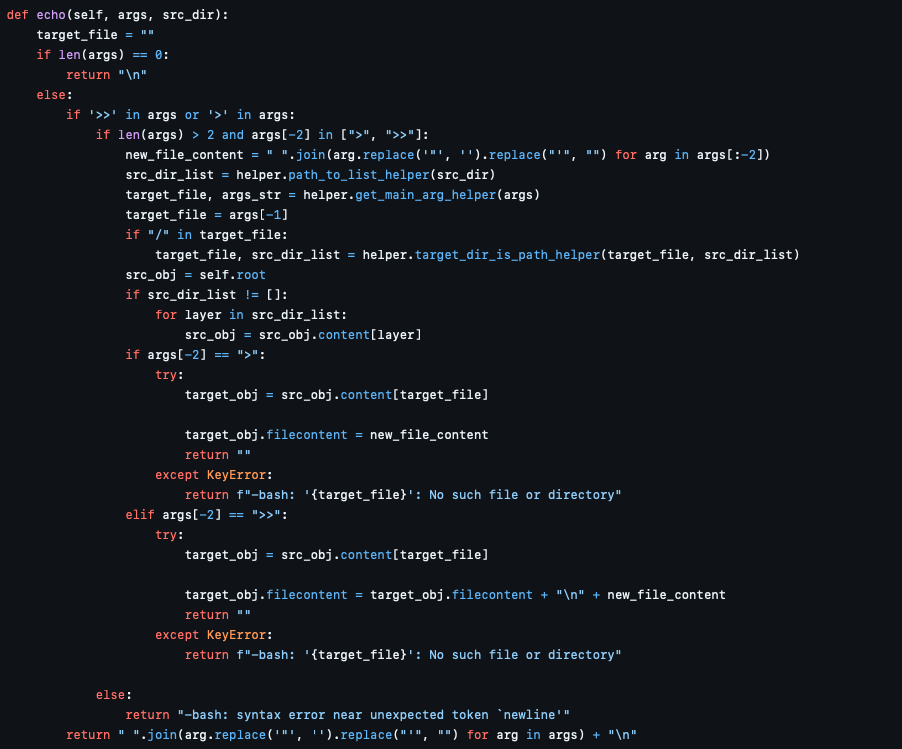
\includegraphics[width=1\linewidth]{bilder/echo_code.PNG}
    \caption{Echo function}
\end{figure}

Problems:

During development, problems often occurred with the ptrace call. A common issue was the error \texttt{No such process}, which appeared when trying to trace a process.

\begin{figure}[H]
    \centering
    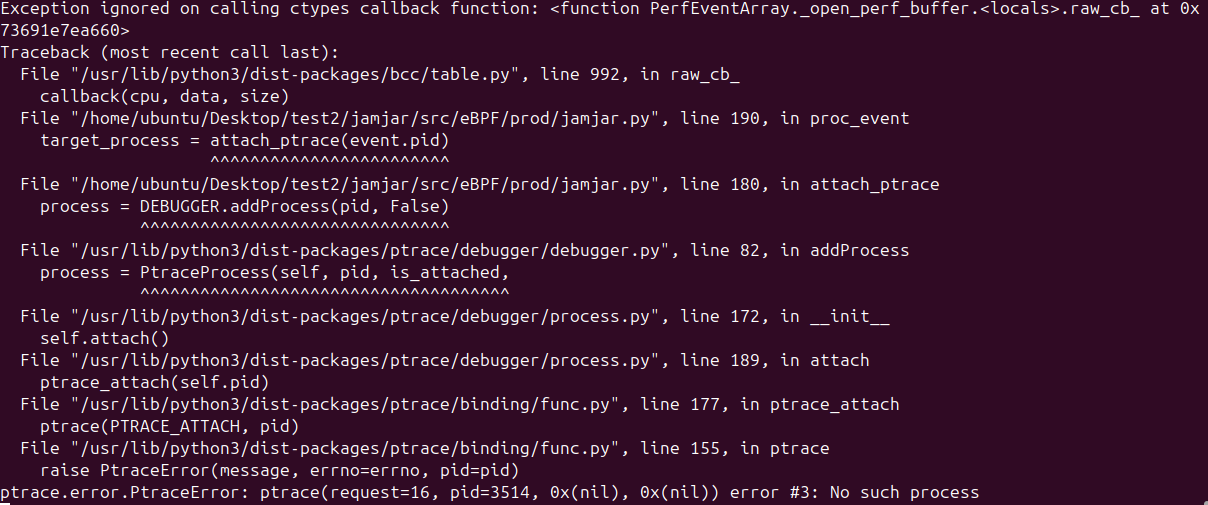
\includegraphics[width=1\linewidth]{bilder/error.PNG}
    \caption{error}
\end{figure}

After analyzing this error, we quickly came to the conclusion that the problems were caused by the short lifespan of the processes. Probably the processes are terminated too quickly so that the ptrace call can no longer be called in time. To check this, we adapted the attach\_ptrace function that throws the error and added some checks:

\begin{figure}[H]
    \centering
    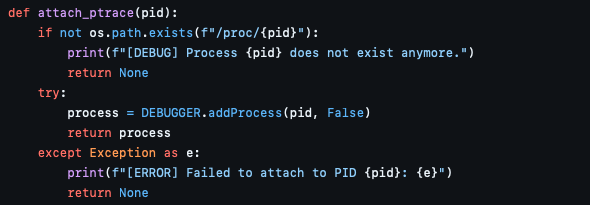
\includegraphics[width=1\linewidth]{bilder/attach_ptrace.PNG}
    \caption{ptrace function}
\end{figure}

This checks whether the process to be terminated still exists at the time of the attach\_ptrace call. If it no longer exists, a suitable message is displayed in the console. If the process is found, the attach\_ptrace function is processed normally.

The results of this adjustment confirmed the assumption, as in some cases the process no longer existed at the time of the attach\_ptrace call.

\begin{figure}[H]
    \centering
    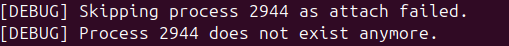
\includegraphics[width=1\linewidth]{bilder/skipping.PNG}
    \caption{ptrace error}
\end{figure}
    \chapter{Results}
\label{chap:results}
\section{Conclusion}
The main goal of this project work was to create a honeypot system for Linux/unix systems that can run on an already-in-use system such as a mailserver of IoT-device. Our solution does provide honeypot capabilities on a system while using only limited resources. Of course this project could not implement all possible unix commands so an attacker will find boundaries and become suspicious when spending enough time on the system. But the open architecture and APIs of JamJar make it easy for others to expand the capabilities by implementing new commands.

\section{Evaluation}
During the presentation the system was shown as a live demo. While a real user can still access the whole system and is not influenced or hindered by JamJar, a potentially breached user account was locked inside the simulated environment and could not easily tell the difference.
As already discussed, currently the simulated environment does contain some abnormalities. For example all files and directories contain the same timestamp and size and all simulated processes use the same amount of CPU and memory. Randomizing these values might be an effective step to make this system more stealthy. Nevertheless JamJar works and because of the lightweight architecture, no noticeable delay between command execution and the simulated response occurs. Also the performance of the host system is not really restricted.

\section{Future Work}
As this project was only the start of JamJar, there are a lot of points and ideas for future work on the topic. For example it might be interesting to be able to replace the simulated system that is loaded into memory on program start in an easy way. We could think of some configuration file stored in JSON format that contains system parameters like the directory structure, running processes or network parameters. Outsourcing these parameters in the configuration file would make it easy to swap them and deploy JamJar on a lot of systems fast. 
Also a separate program could be implemented to generate this configuration from another machine simply be executing it on the running system. This would allow JamJar to generate some sort of fingerprint of machines that can be used as the configuration file.

Another interesting approach might be the simulation of a windows system. Although the currently used commands and technologies such as eBPF are not as easily accessible on Windows machines, there is also a need for honeypot systems in windows environments.


    % ------------------------------------------------------------------
    
    \label{lastpage}
    
    % Neue Seite
    \cleardoublepage
    
    % Backmatter mit normalem Zeilenabstand setzen
    \singlespacing
    
    % Römische Ziffern für die "Back-Matter", fortlaufend mit "Front-Matter"
    \pagenumbering{Roman}
    \setcounter{page}{\value{frontmatterpage}}
    %\setcounter{page}{0}

    % Abkürzungsverzeichnis
    \cleardoublepage
    \phantomsection
    \printnoidxglossary[type=\acronymtype,title=List of Abbreviation,nonumberlist]
    \printnoidxglossary[title=Glossary,nonumberlist]
    
    % Tabellenverzeichnis erzeugen
    \cleardoublepage
    \phantomsection
    \addcontentsline{toc}{chapter}{\hsmalistoftables}
    \listoftables
    
    % Abbildungsverzeichnis erzeugen
    \cleardoublepage
    \phantomsection
    \addcontentsline{toc}{chapter}{\hsmalistoffigures}
    \listoffigures
    
    % Listingverzeichnis erzeugen - Quellcode falls vorhanden
    %\cleardoublepage
    %\phantomsection
    %\addcontentsline{toc}{chapter}{\hsmalistings}
    %\lstlistoflistings
    
    %Literaturverzeichnis erzeugen
    \begin{flushleft}
        \printbibliography
    \end{flushleft}
        
    % Index ausgeben. Wenn Sie keinen Index haben, entfernen Sie einfach diesen Teil.
    %\cleardoublepage
    %\phantomsection
    %\addcontentsline{toc}{chapter}{\hsmaindex}
    %\printindex
    
    % Anhang. Wenn Sie keinen Anhang haben, entfernen Sie einfach
    % diesen Teil.
    %\appendix
    %\chapter{Anhang A}\label{anhang:a}

\end{document}
